%%%%%%%%%%%%%%%%%%%%%%%%%%%%%%%%%%%%%%%%%%%%%%%%%%%%%%%%%%%%%%%%%%%
%                                                                 %
%                            ROOT FILE                            %
%                                                                 %
%%%%%%%%%%%%%%%%%%%%%%%%%%%%%%%%%%%%%%%%%%%%%%%%%%%%%%%%%%%%%%%%%%%
%
%  Run LaTeX or pdfLaTeX on this file to produce your thesis.
%  To produce the abstract title page followed by the abstract,
%  see the file abstitle-phd.tex or abstitle-mas.tex.
%
%%%%%%%%%%%%%%%%%%%%%%%%%%%%%%%%%%%%%%%%%%%%%%%%%%%%%%%%%%%%%%%%%%%

\documentclass[chap]{thesis}

%%%%%%%%%%%%%%%%%%%%%%%%%%%%%%%%%%%%%%%%%%%%%%%%%%%%%%%%%%%%%%%%%%%

\usepackage{graphicx}
\graphicspath{ {resources/} }

%\usepackage{amsmath}
%\usepackage{amsthm}
%\usepackage{amssymb}
\usepackage[usenames,dvipsnames,svgnames,table]{xcolor}
\usepackage{pdfpages}
\usepackage{tikz}
\usepackage{amsmath}
\usepackage{amssymb}
\usepackage[numbers]{natbib}
\usepackage[labelfont=bf]{caption}
\usepackage[labelformat=simple]{subfig}
\usepackage{mathtools}


\usepackage{mathpazo}
\usepackage[chapter]{algorithm}
\usepackage[noend]{algpseudocode}

% \renewcommand{\thechapter}{\Roman{chapter}}
% \renewcommand{\thesection}{\arabic{section}}
% \renewcommand{\thealgorithm}{\arabic{chapter}.\arabic{algorithm}} 

\DeclarePairedDelimiter\ceil{\lceil}{\rceil}
\DeclarePairedDelimiter\floor{\lfloor}{\rfloor}

\newcommand*{\head}[1]{%
	\textbf{#1}
}
\newcommand{\cnote}[1]{%
	{\color{red}[#1]}
}
\renewcommand{\textfraction}{0.01}
\renewcommand{\floatpagefraction}{0.99}
\renewcommand{\topfraction}{0.99}
\renewcommand{\bottomfraction}{0.99}
\renewcommand{\dblfloatpagefraction}{0.99}
\renewcommand{\dbltopfraction}{0.99}
\renewcommand{\th}{$^{th}$}
\newcommand{\conv}{\mathop{\scalebox{1.2}{\raisebox{-0.2ex}{$\ast_{x,y}$}}}}

%%%%%%%%%%%%%%%%%%%%%%%%%%%%%%%%%%%%%%%%%%%%%%%%%%%%%%%%%%%%%%%%%%%

\begin{document}
    %%%%%%%%%%%%%%%%%%%%%%%%%%%%%%%%%%%%%%%%%%%%%%%%%%%%%%%%%%%%%%%%%%%
%                                                                 %
%                            TITLE PAGE                           %
%               Master's Thesis or Master's Project               %
%                                                                 %
%%%%%%%%%%%%%%%%%%%%%%%%%%%%%%%%%%%%%%%%%%%%%%%%%%%%%%%%%%%%%%%%%%%

% Supply information for use on title page:
\thesistitle{\bf Sketch Based Interface for\\ Architectural Design}
\author{Eric\ Zhang}
\degree{Master of Science}
\department{Computer Science}

\signaturelines{3}
\projadviser{Dr. Barbara Cutler}
\memberone{Dr. Charles Stewart}
\membertwo{Dr. Randolph Franklin}

\submitdate{July 2016\\(For Graduation August 2016)}
\copyrightyear{2016}   % if omitted, current year is used.

% Print titlepage and other prefatory material:
\titlepage
\copyrightpage         %optional
\tableofcontents
\listoftables          %required if there are tables
\listoffigures         %required if there are figures

    \newpage
    %%%%%%%%%%%%%%%%%%%%%%%%%%%%%%%%%%%%%%%%%%%%%%%%%%%%%%%%%%%%%%%%%%%
%                                                                 %
%                         ACKNOWLEDGEMENTS                        %
%                                                                 %
%%%%%%%%%%%%%%%%%%%%%%%%%%%%%%%%%%%%%%%%%%%%%%%%%%%%%%%%%%%%%%%%%%%

\specialhead{ACKNOWLEDGMENTS}

I would like to thank my thesis adviser, Dr. Barbara Cutler, for her thoughtful advice, experience, and feedback throughout the creation of this thesis. I would like to thank my lab mates Max Espinoza, Sensen Chen, Jim Olyha, and Jeramey Tyler for their helpful suggestions and criticism of my work. I would also like to thank all of my friends I've met at RPI, for they've made my experience here all the more worthwhile. Finally, I'd like to thank my parents, Weixian Zhang and Popo Chan, for their unwavering support throughout my education, for without them none of this would be possible.

    \newpage
    %%%%%%%%%%%%%%%%%%%%%%%%%%%%%%%%%%%%%%%%%%%%%%%%%%%%%%%%%%%%%%%%%%%
%                                                                 %
%                            ABSTRACT                             %
%                                                                 %
%%%%%%%%%%%%%%%%%%%%%%%%%%%%%%%%%%%%%%%%%%%%%%%%%%%%%%%%%%%%%%%%%%%
\specialhead{ABSTRACT}

The use of sketching amongst architects contributes  significant benefits in the creation of creative and professional projects. Sketching offers a simple method of conveying ideas to an audience, without a large time commitment. As a result, architects can prototype designs rapidly, exploring many patterns while receiving feedback on their work. Sketching influences the design process by allowing the designer to work more creatively and effectively through quick, numerous iterations. The use of sketching in architectural design interfaces has only increased the flexibility and possible designs for users. However, variation in human input increases the difficulty to accurately recognize the intent of the user. Traditional methods of interacting with architectural design interfaces rely on creation of fixed sized primitives. When interacting with such systems, design options feel more limited. \\

I present an alternative sketch-based interface for the Online Architectural Sketching Interface for Simulations. This interface emulates drawing using paper and pencil, allowing the user to create lines on a canvas. Using the user input, the interface recognizes certain series of strokes as objects, creating furniture items as feedback to the user. The strokes are also processed by the system as different gestures, allowing the user a multitude of options to edit designs. \\

%Using these shapes, the system classifies them as possible furniture items.

Contributions of this thesis include the development of an architectural sketching interface, algorithms to perform recognition and fitting of interface primitives, and conduction of a pilot study. 
%%%%%%%%%%%%%%%%%%%%%%%%%%%%%%%%%%%%%%%%%%%%%%%%%%%%%

    %%%%%%%%%%%%%%%%%%%%%%%%%%%%%%%%%%%%%%%%%%%%%%%%%%%%%%%%%%%%%%%%%%%
%                                                                 %
%                            CHAPTER ONE                          %
%                                                                 %
%%%%%%%%%%%%%%%%%%%%%%%%%%%%%%%%%%%%%%%%%%%%%%%%%%%%%%%%%%%%%%%%%%%

\chapter{INTRODUCTION} \label{sec:introduction}

A sketch is a rough or unfinished drawing that represents the essential features without all the details. However, the absence of detail in a sketch does not make it less significant than a finished drawing. Sketches allow designers to express their ideas to others in a quick manner, without committing themselves fully. The agile nature of sketches also allow designers to rapidly prototype many ideas while receiving feedback on their work. With this combination of traits, sketching becomes the ideal method of exploring and refining new ideas. \\

The purpose of sketching is twofold: to convey ideas to others and to explore new designs. It is simple to imagine a concept in your head for yourself, it is a completely different challenge to communicate that concept to another person. The ability to effectively communicate your ideas to a client or peers is invaluable in saving time and stimulates productive conversation on the design itself. Sketching is helpful in getting across basic elements about an idea without spending too much time on smaller details. Due to the speed at which sketches can be produced, a designer can afford to explore new, untested ideas. The designer can then aggregate the best qualities, or learn what to avoid in future designs. The two purposes of sketching are closely related and can used to build off one another.

\section{Architectural Drawings and Sketches}
Architects create many sketches and drawings when designing a structure, each with varying degrees of detail. Each image serves its own purpose and has its place within the architectural design process. Sketches are appropriate earlier in the design process when an image's main purpose is to express the architect's design and meet the owner's goals and expectations, while drafts are more appropriate later in the process when contractors need to approximate cost and physically construct the building. Typically, as the process progresses, the level of detail increases. As more details are finalized, and less pieces of the design are left to interpretation.

\subsection{Sketches}

\begin{figure}[ht]
\centering
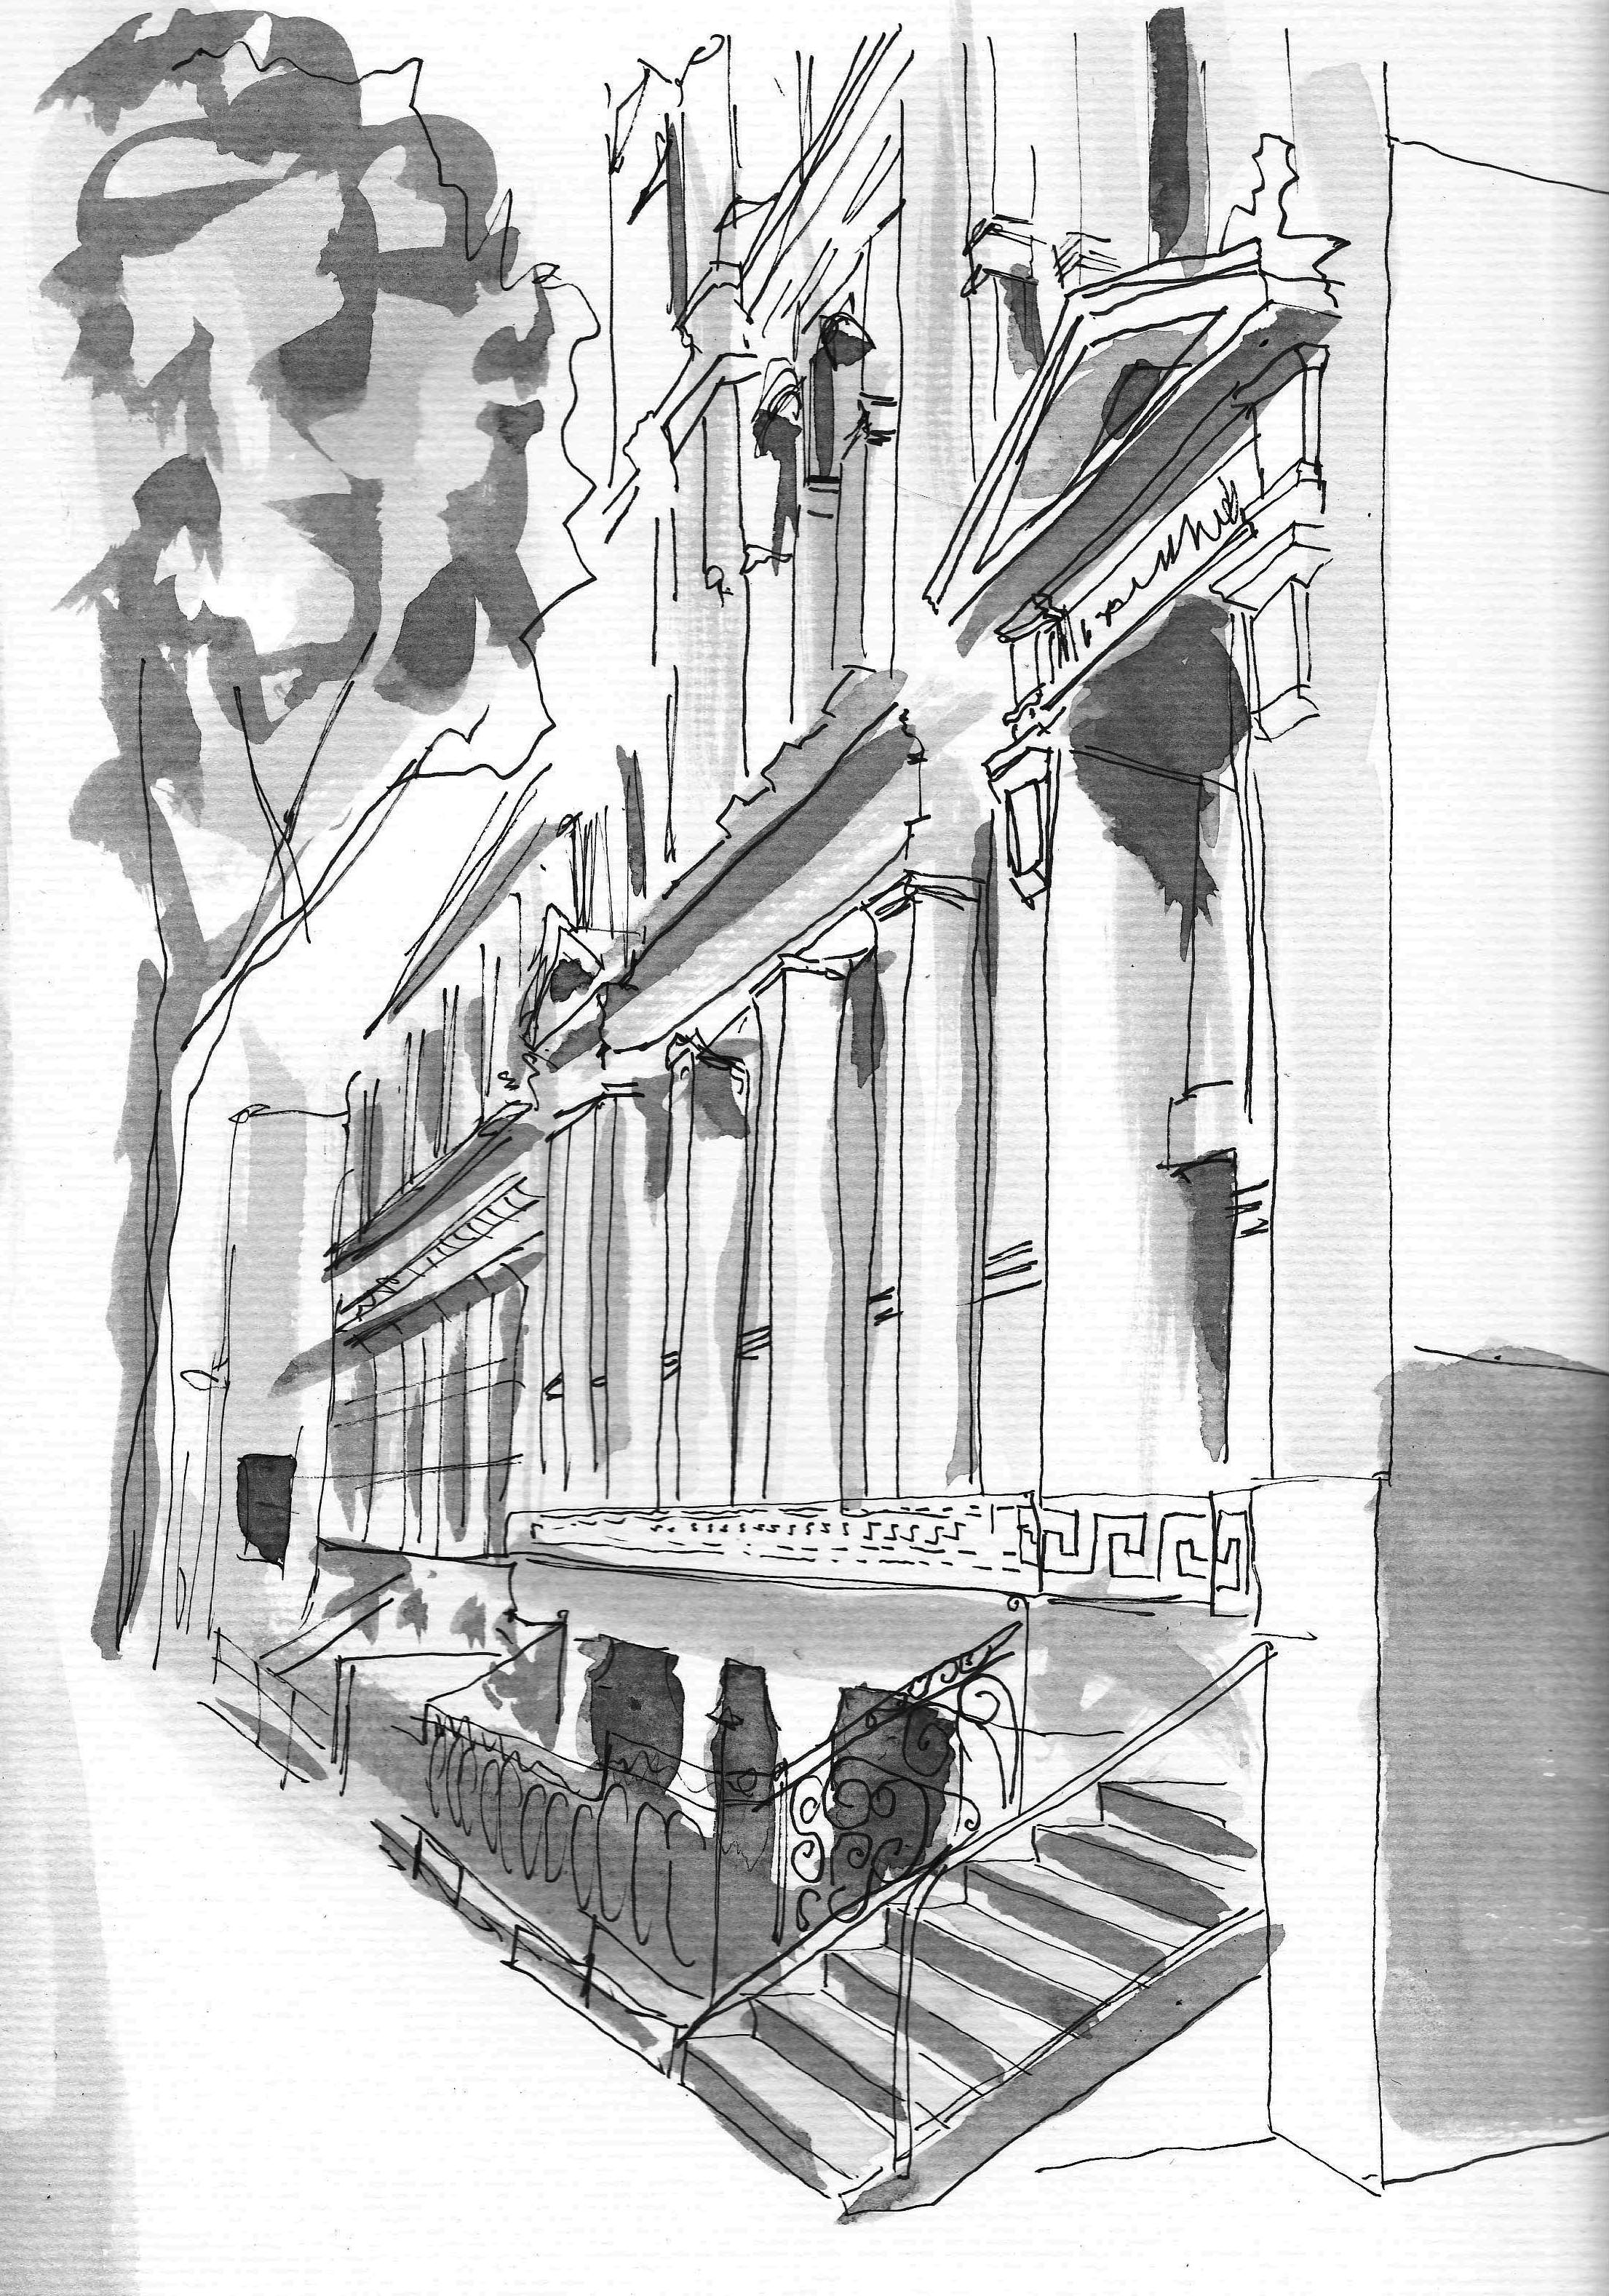
\includegraphics[width=.6\textwidth]{quicksketch}
\caption[Example of a quick architectural sketch.]{A quick sketch depicting the front view of the Lombard Building on Queen Street, Melbourne. Sketched by Aushist, used under GNU Free Documentation License \cite{quicksketch}.}
\label{fig:quicksketch}
\end{figure}

Sketches are among the most basic drawings created by architects. Their simplicity in creation and design allow for quick modification of ideas and ease of understanding of general concepts. No initial sketch needs to have correct scale or the dimension numbers, as long as the ideas of the designer reach his or her intended audience. Without too much detail, audience can focus on the key details the designer has purposefully chosen to include in the sketch. A sketch is the perfect vehicle for rapid prototyping and design analysis, without the accuracy and time commitment required for producing a draft. \\

\begin{figure}[ht]
\centering
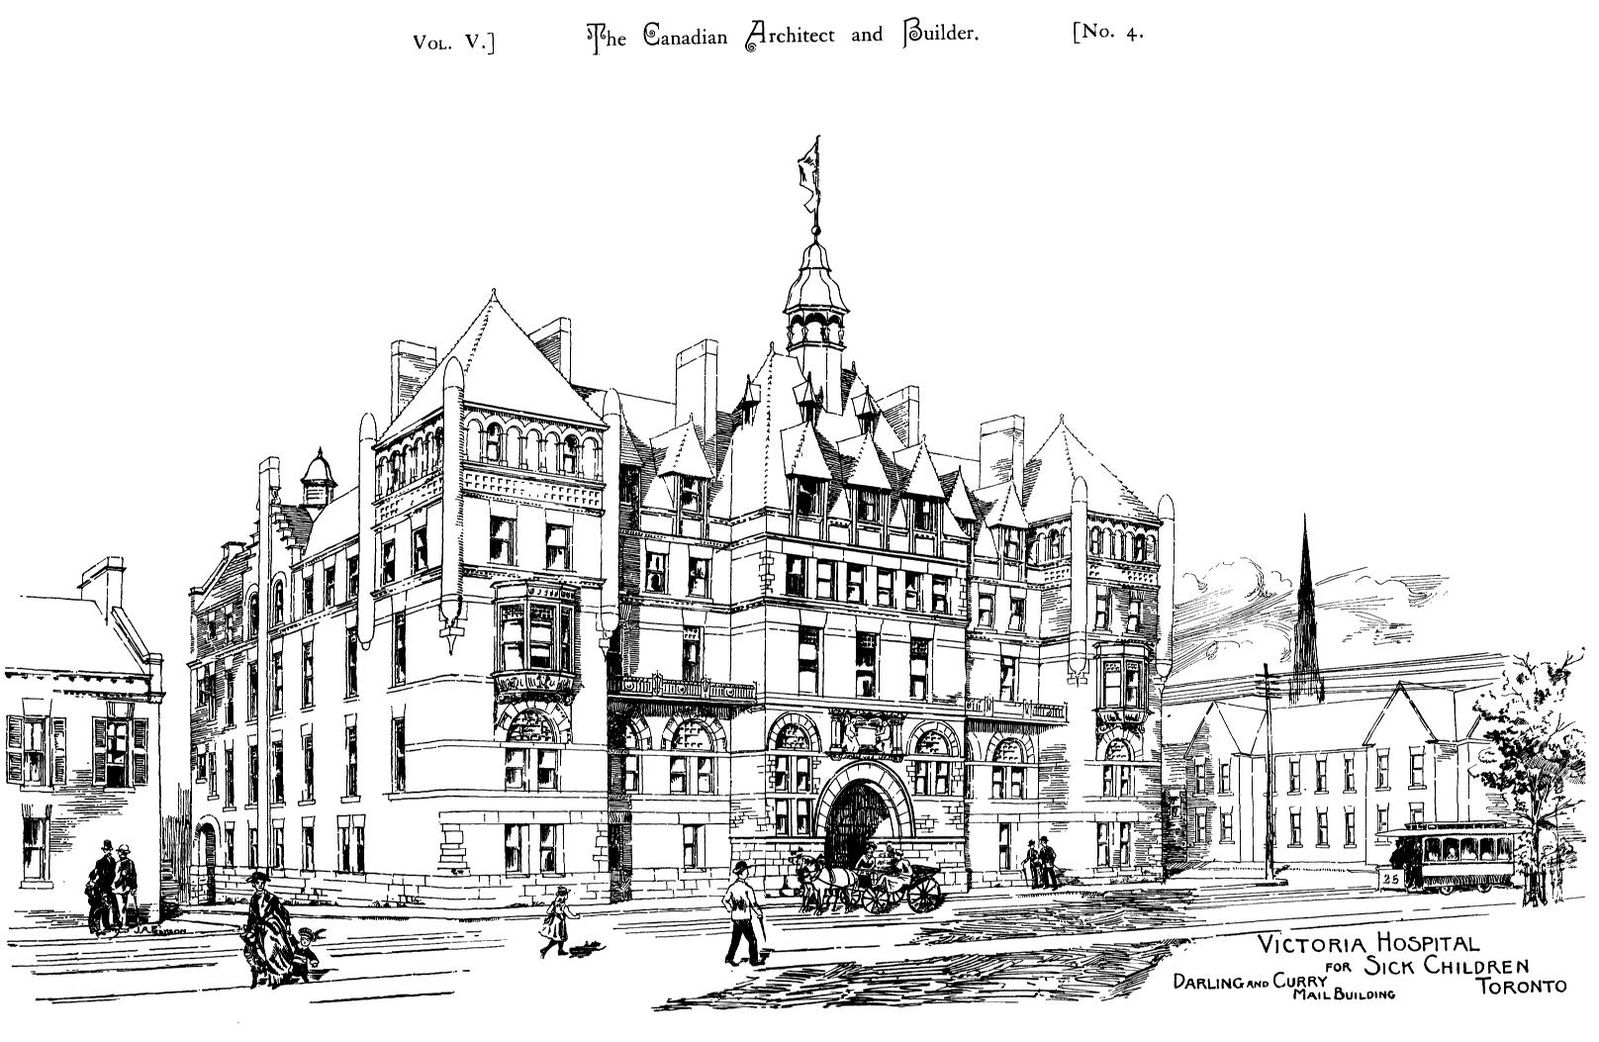
\includegraphics[width=\textwidth]{archsketch}
\caption[Example of an architectural sketch - elevation view]{An architectural sketch of the elevation view depicting the Victoria Hospital for Sick Children. Drawn by Darling and Curry work is in public domain \cite{hospital}.}
\label{fig:archsketch}
\end{figure}

Depending on what needs to be shown, architects can sketch their design from many different angles \cite{drafting_and_design}. A floor plan is the fundamental view for a building. It displays the layout of the building at a certain elevation, showing details on a floor by floor basis, as shown in Figure \ref{fig:topdownsketch}. For a side view the interior, an architect can construct a cross section view. A cross section view is an image of the building from the side, cut by a plane. It shows the relationship between different floors, and how they are layered on top of each other. If a client wants to see how a building appears from the outside, the architect can present an elevation view, such as the one illustrated in Figure \ref{fig:archsketch}. An elevation view is a flat view from the outside of building at a certain height, showing one face of the structure. Since most buildings are not the same at all angles, elevation views from multiple angles may be constructed. One particular angle is an isometric angle, which is a view where the angles between the projections of all axes are equivalent. As shown in the left image in Figure 1.1, an isometric view displays the outside only, and shows the connections between outside elements. To show the context around where a building is located, a site plan is created. It is an overhead view, similar to a floor plan, but it displays the whole property instead of one building. When designing a building, an architect will create most, if not all, of these views to present to the owner so he/she can accurately understand the architect's ideas.

\subsection{Drafting}

Before an architect's design can become a building, architectural drafts of the design need to be created. Drafts are extremely high detail drawings depicting dimensions, structure, and layout of a building \cite{drafting_and_design}. There exists drafts of many aspects of the building, such as electrical, plumbing, and structural. These drafts help guide the contractors to construct the building according to the design and specifications set by the architect and owner. Before the existence of computer-aided drafting (CAD) software, drafts were created meticulously by hand. Drafts were checked by many people; small mistakes could have massive consequences on the structure of a building. 

\begin{figure}[ht]
\centering
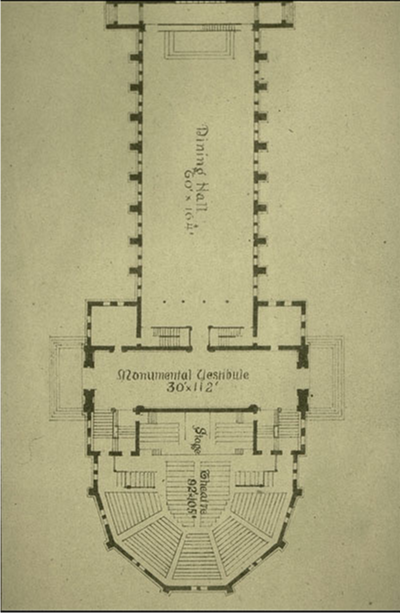
\includegraphics[width=.8\textwidth]{rotated}
\caption[Example of a hand drawn architectural sketch - floorplan]{A hand drawn architectural floorplan of Memorial Hall (Harvard University). Author unknown, work is in public domain \cite{harvard}.}
\label{fig:topdownsketch}
\end{figure}

% AutoCAD SolidWorks NX

With the rise of computing power through the 1970's and 1980's, so too did the benefits of switching over to computer-aided drafting (CAD). CAD software drastically increased the quality of designs produced, improved communication between architects and engineers, and boosted productivity \cite{cad}. CAD software creates more accurate drafts, without object scales needing to be manually verified. Control over information about structure, electricity, plumbing and much more are all organized and displayable on a whim. Editing the project is no longer as tedious; objects can be deleted, copied, rotated, and scaled, with few button clicks. The benefits of using CAD software are immense, and its prevalence in fields such as architecture and engineering reflects that.

\begin{figure}[ht]
\centering
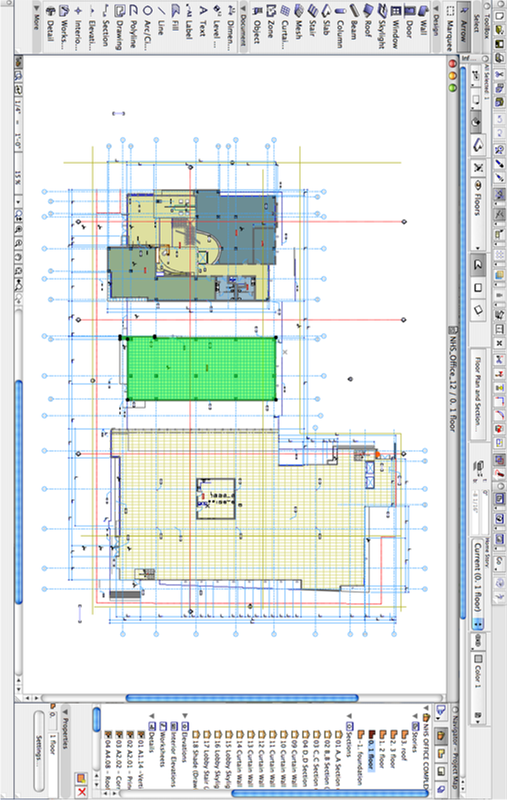
\includegraphics[width=.75\textwidth]{cadrotate}
\caption[Example of a room designed using CAD software]{An example floor plan created using ArchiCAD \cite{archicad}. Created by Martinremco, work is used under Creative Commons \cite{cad1}.}
\label{fig:cad1}
\end{figure}

The sheer strength of the tools available with CAD software dwarfs the power of a person with pencil and paper, and the drawings produced by both mirrors that imbalance. To produce a draft with the same quality, a hand drawn model would take a great deal more time and effort compared to one created with software. Using tools such as AutoCAD \cite{autocad}, ArchiCAD \cite{archicad}, and NX \cite{nx}, designers have more power than ever. Figure \ref{fig:cad1} illustrates one example of a design using ArchiCAD. However, using CAD software is not without its downsides. Compared to drawing on paper, a large amount of training or familiarity with the program is required to proficiently create drafts. Improper use of software can be a hindrance when designing, making other tasks more difficult. Since software is constantly changing, there continues to be more learning required, especially with large updates or feature changes. Despite all the drawbacks, CAD software continues to be a leading choice for many architects and engineers.

\section{The Architectural Design Process}

Architects often follow a five step process from design to completion of a building. The five phases are: schematic design, design development, construction documents, bid or negotiation, and construction administration \cite{bestpractices}. During the schematic design phase, the architect and client work together to determine the goals and needs of the project. The architect creates drawings and documents to accurately show their concept to the owner. He or she also researches zoning and jurisdictional restrictions to present to the client. At the end of this phase, the architect will produce a final schematic design that will be the basis for cost, design, and development. Next, during the design development phase, details for multiple elements of the building are finalized, including windows, walls, and doors. Structural details such as plumbing and electrical are also settled upon. After, the construction documents are created with the information from the design development phase. A schematic design is created with even greater detail for contractors to pricing and bidding. Afterwards, bids and negotiation begin for the construction of the building. The owner and architect will review bids and select a contractor to construct the building. Finally, the construction begins on the project. Though out construction of the building, The architect will continue to help the contractor build the project as specified in the documents created during the construction documents phase. \\

% We focus primarily on the the earliest portion of the schematic design phase. 

Design plays a crucial role in the architectural design process. Each phase builds off the work done in previous stages, so the design done during the schematic design phase is the foundation for the rest of the project. Our focus in this thesis work is to improve the schematic design phase of the architectural design process. We hope to facilitate more efficient exploration of new ideas, as well as a smoother transition into the next phase.

\section{Benefits of Sketching in Design}

% Sketching typically occurs during the infancy of any project, whether it be a piece of artwork or schematics for a building. This phase is often called the design phase. The ideas and thoughts manifested during this phase are the foundation for what is created in later phases.

% Design, or inception of an idea, is often the first step in creating a successful building. Good design is a combination of many features: usefulness, aesthetics, and so on.

The term "design" can be used to describe many different actions or creations across many fields. References can be drawn to graphic design in art, engineering design, the design of computer code, design of production processes, even the process of design itself \cite{howdesignersthink}. In some cases, design can be construction of the object itself, such as a piece of artwork. In essence, design is the manifestation of an idea into a plan or drawing to accomplish some task or goal. For example, when tasked with designing a website, I sketched out some designs before constructing anything. The results are show in Figure \ref{fig:websitesketch}. Being able to design well means merging individual components together cohesively to accomplish some objective. Achieving the goal in the most efficient and elegant way possible is the ambition of all designers. \\

\begin{figure}[ht]
\centering
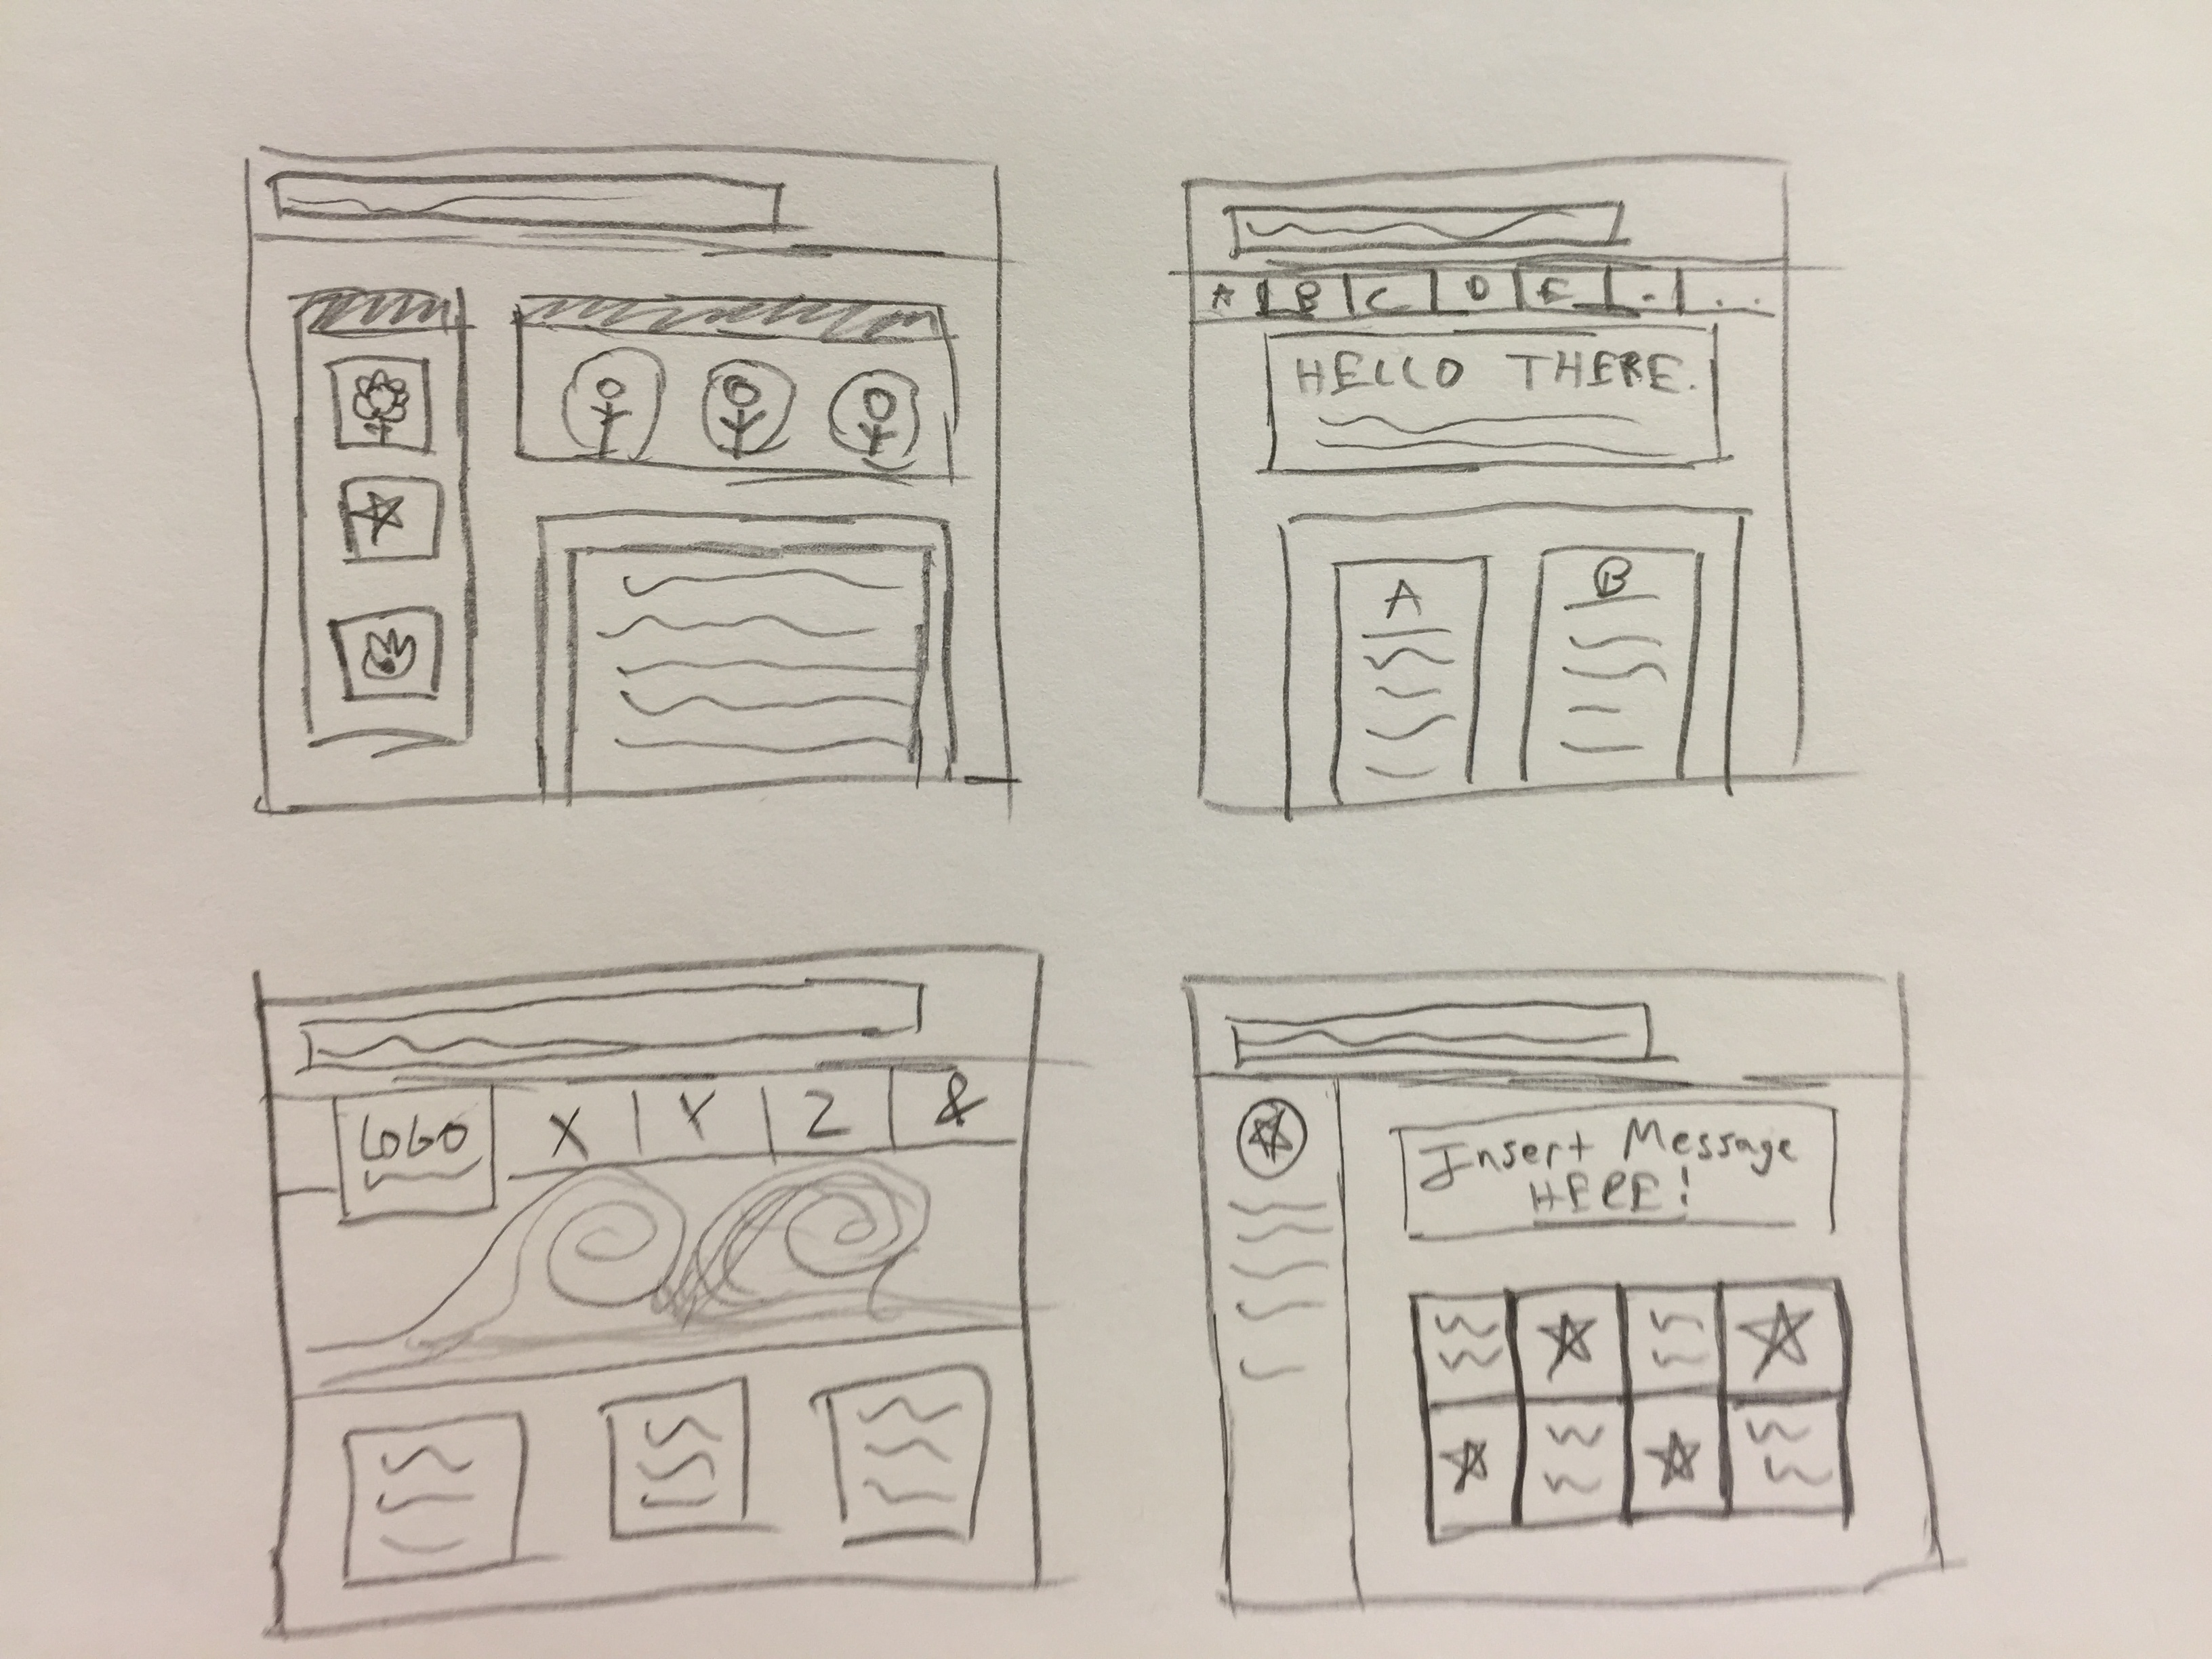
\includegraphics[width=\textwidth]{webdrawing}
\caption[Design sketch examples drawn when tasked with designing a website.]{Sketches drawn when tasked with designing a website.}
\label{fig:websitesketch}
\end{figure}

There are many benefits to sketching ideas when designing. Throughout the design process, sketching is invaluable for communicating ideas \cite{ullmanwood1990}. Sketching is a self reflective process, and allows for the designer to efficiently map out their thoughts in a manner that makes more sense \cite{howdesignersthink}. Seeing, moving, improving their designs helps users increase their design proficiency \cite{schon2004}. Song and Agogino \cite{song2004} observed that there was a positive correlation between usage of sketches and the user's design outcome. The process of making sketches to solve problems also induces a 'design reasoning' that increases visual thinking and puzzle solving \cite{dialects}. Studies have shown that not only did sketching allow the designer to think more creatively, it also stimulated the clients those designers were working for \cite{Schutze2003}.  When sketching, designers more often than not changed their original ideas and formed new ones, while those who used a drawing program were more limited in what they created. There have been positive correlations found between number of designs and the outcome, as observed by Yang \cite{yang2009}. In the early design process, self made sketches increased the quality of solutions proposed, as well as having an overall positive impact on the final product. Users who had the opportunity to sketch their ideas in the design phase found the problems to be significantly easier and this solution quality increased \cite{Schutze2003}. These user thought the solution was much more intuitive and were able to logically progress through a solution more quickly for the problem at hand. \\

A similar process can be used in architectural sketching implementations. The ability to sketch out ideas can have a positive impact on the overall end product. The importance of sketching to an architect cannot be understated. Sketching as a tool has been observed to be valuable when used for creative tasks \cite{Schutze2003}. Utilizing the creative power of sketching, we aim to create an interface that improves the design potential of all its users.

\section{Thesis Outline and Contributions}

This thesis is motivated by the creation of the Online Architectural Sketching Interface for Simulations (OASIS) \cite{oasis2016}. There was a desire to create a more novel, cohesive, and intuitive way to design models. The previous iteration of OASIS utilized a drag-and-drop user interface for creating designs. To improve the system, imitating how architects design buildings seemed like the most logical option. Architects design buildings first on pencil and paper, then transition to a CAD program to add further detail. By accepting inputs as strokes, we hope to give the user freedom and flexibility that was not available in the previous iteration. \\

The first step in creating a solution that met our goals was to create a process that accepted user input in the form of strokes. Chapter 2 outlines some of the work leading up to the creation of this sketching interface. Next, chapter 3 explains the pipeline of OASIS, how this work modifies and improves previous features, and basic elements of the interface. Chapters 4 details how the system uses the simple strokes input by the user to create a design that matches the user's intentions. Chapter 5 includes a small informal pilot study on the usage of the current interface against the previous one. Finally, chapter 6 concludes with closing remarks and potential directions for further improvements and research.
    %%%%%%%%%%%%%%%%%%%%%%%%%%%%%%%%%%%%%%%%%%%%%%%%%%%%%%%%%%%%%%%%%%%
%                                                                 %
%                            CHAPTER TWO                          %
%                                                                 %
%%%%%%%%%%%%%%%%%%%%%%%%%%%%%%%%%%%%%%%%%%%%%%%%%%%%%%%%%%%%%%%%%%%
\chapter{RELATED WORKS} \label{sec:related}
%talk about the main topic of your thesis, and a blurb about what is related

Sketch interpretation on a computer interface is not trivial to implement. While recording user input is not difficult, it is challenging to interpret the user's intent correctly. Drawings and sketches created by users are often ambiguous and difficult to understand for an application. The minute differences between user actions can result in the system returning vastly different outcomes. Higher degrees of accuracy often require large amounts of data, demanding higher computer specifications to execute properly. With greater resources demanded, it becomes increasingly difficult for sketch interpretation to become available for widespread use. \\

% This thesis provides an alternative sketching interface for the online architectural sketching interface for simulations (OASIS). The OASIS is an architectural sketching application designed for early design prototyping \cite{oasis2016}. Using OASIS, users can create daylight simulations based on user-designed models. 

In this chapter, I will outline some work done on OASIS prior to the development of this sketching interface. We will also discuss some related works regarding sketch recognition, and its applicability to this application. Finally, we discuss some related software and their approaches to reaching similar goals.

%PICTURES OF OASIS
%PICTURES OF OASIS
%PICTURES OF OASIS

\section{OASIS}

OASIS is an online architectural sketching application developed by fellow colleague, Max Espinoza \cite{oasis2016}. Its primary purpose is to generate closed 3D meshes with optimal properties for simulations. OASIS is an alternative form of the Virtual Heliodon, a tangible user interface for daylighting simulation \cite{yusheng}.  Currently, OASIS only supports simulating daylight visualizations \cite{oasis2016}. To begin, users create 2D floor plans using the design interface. Next, OASIS interprets and constructs 3D models based on the designs. Finally, the tasks may be generated with various parameters and executed on one of our servers.

\begin{figure}[ht]
\centering
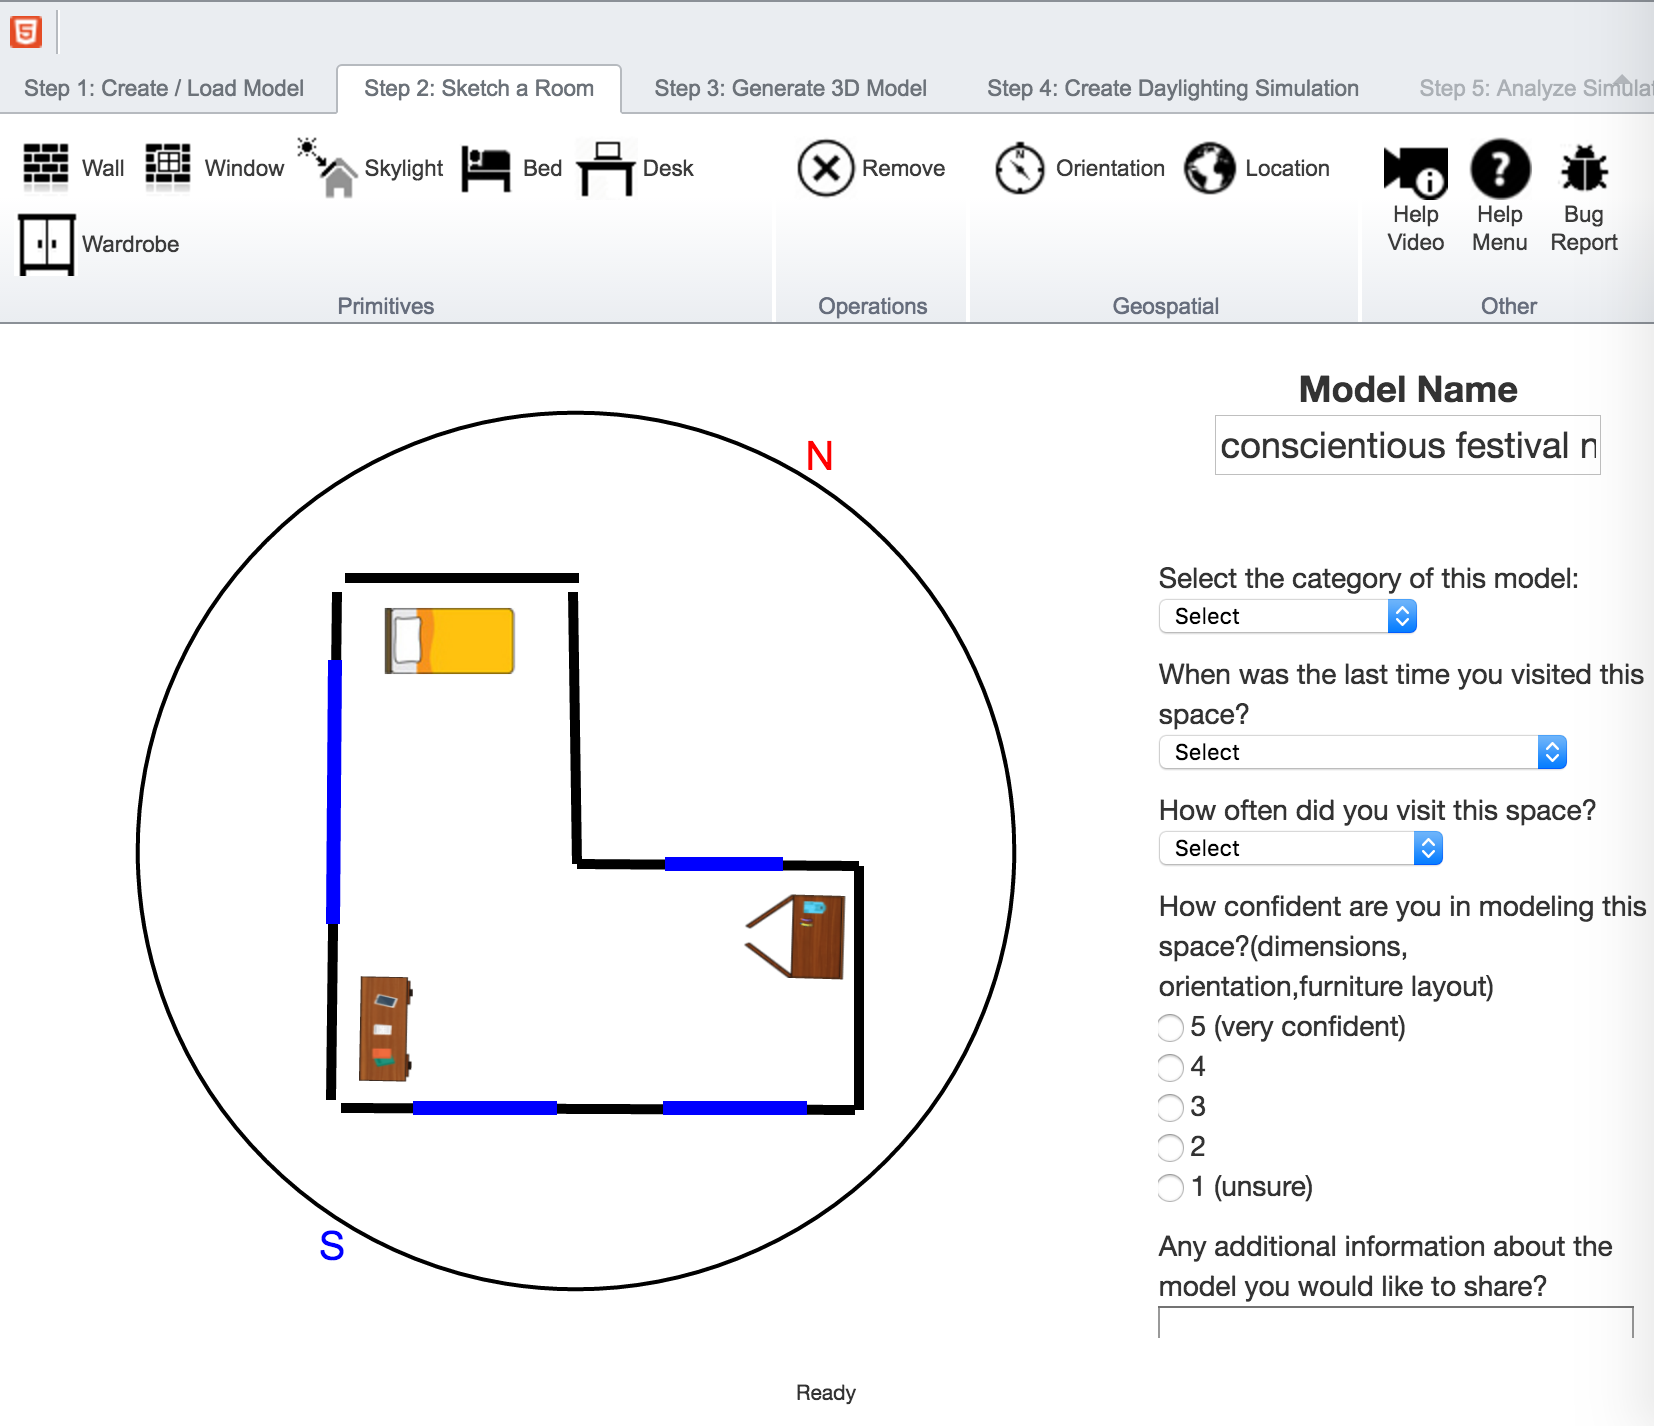
\includegraphics[width=\textwidth]{oasis}
\caption[Image of the sketching interface used in OASIS]{Image of the sketching interface used in OASIS \cite{oasis2016}.}
\label{fig:oasis}
\end{figure}

There are many design choices available when creating a sketch on OASIS. Users can create walls, windows, beds, desks, and wardrobes. All furniture items are editable and easily configurable. Along with basic primitives, a cardinal orientation for the room may be chosen, as well as any location in the world. When creating daylighting tasks, users have options when simulating the environment surrounding their rooms. Tasks are editable with dates, times, timezones, and weather condition. Users also have the option to share their models with others via URL \cite{oasis2016}. A unique link can be shared with family and friends to show off designs and gather feedback. Overall, OASIS provides a wide array of choices for users to personalize their designs.

\section{Previous Work on OASIS}

My contributions to OASIS are not limited to the creation of the new sketching interface. Before the inception of this work, I developed features and fixed bugs to improve user experience on OASIS. The time spent improving the application was invaluable for gaining familiarity with the system and learning about the development process. Using OASIS also helped me realize some of its flaws, which helped inspire the creation of this thesis. Without this prior experience, developing a new sketching interface would have been far more difficult. \\

One contribution was the implementation of a Cron job to regularly select tasks. Cron is a time based scheduler in Unix-based systems that runs commands at preset intervals \cite{cron}. The implemented Cron job is set to check user submissions at short intervals for newly submitted tasks, and execute them using the daylight simulation rendering engine. Before the implementation of the Cron job, there was no method to select one task over another task, and tasks were run when they were submitted. This could cause problems overloading the server if too many tasks were queued at the same time. The importance of the Cron job is to give the system control over which task will be processed next. Currently, the script selects based on first-come-first-serve. However, the selection process could be improved in the future to increase fairness between users. For example, if a User A enters the queue while User B has 100 tasks already in queue, it would be unfair for User A's task to be the 101st task processed, even if it was the 101st task created. \\

The task tab is where the user can create daylighting simulation tasks for our server to process. I made a number of improvements to the task tab to improve user experience, including dynamic sizing of the table, additional information about the tasks themselves, improved readability, and automatic timezone estimation. Timezone estimation is based on the user's choice of location when designing using the sketching interface. Based on the x and y coordinates of the location selection, I estimate which timezone it is closest to, and automatically select that timezone when a user creates a new task. \\

In daylighting simulations, the importance of windows cannot be understated, since the illumination of the room is entirely based on windows. Consequently, there is a high priority for windows to be designed correctly. One enhancement to the old sketching interface composed primarily of improved window snapping. In OASIS, windows are created by switching into window mode and drawing a stroke near a wall, snapping the window directly onto the wall. There existed minor issues involving the creation of walls with zero or infinite slope. If a user created a window and attached it to a wall with a zero or infinite slope, the window would snap to the maximum length of the wall, regardless of its intended length. The behavior for wall snapping was improved to attach only to the nearest wall with a relatively similar slope to the window drawn, with a maximum length of 90 percent of the wall (5 percent extra room on both ends), and to snap a window of the user's intended length regardless of the slope of the wall. This wall creation procedure heavily influenced the creation of windows in the new sketching interface. \\

\begin{figure}[ht]
\centering
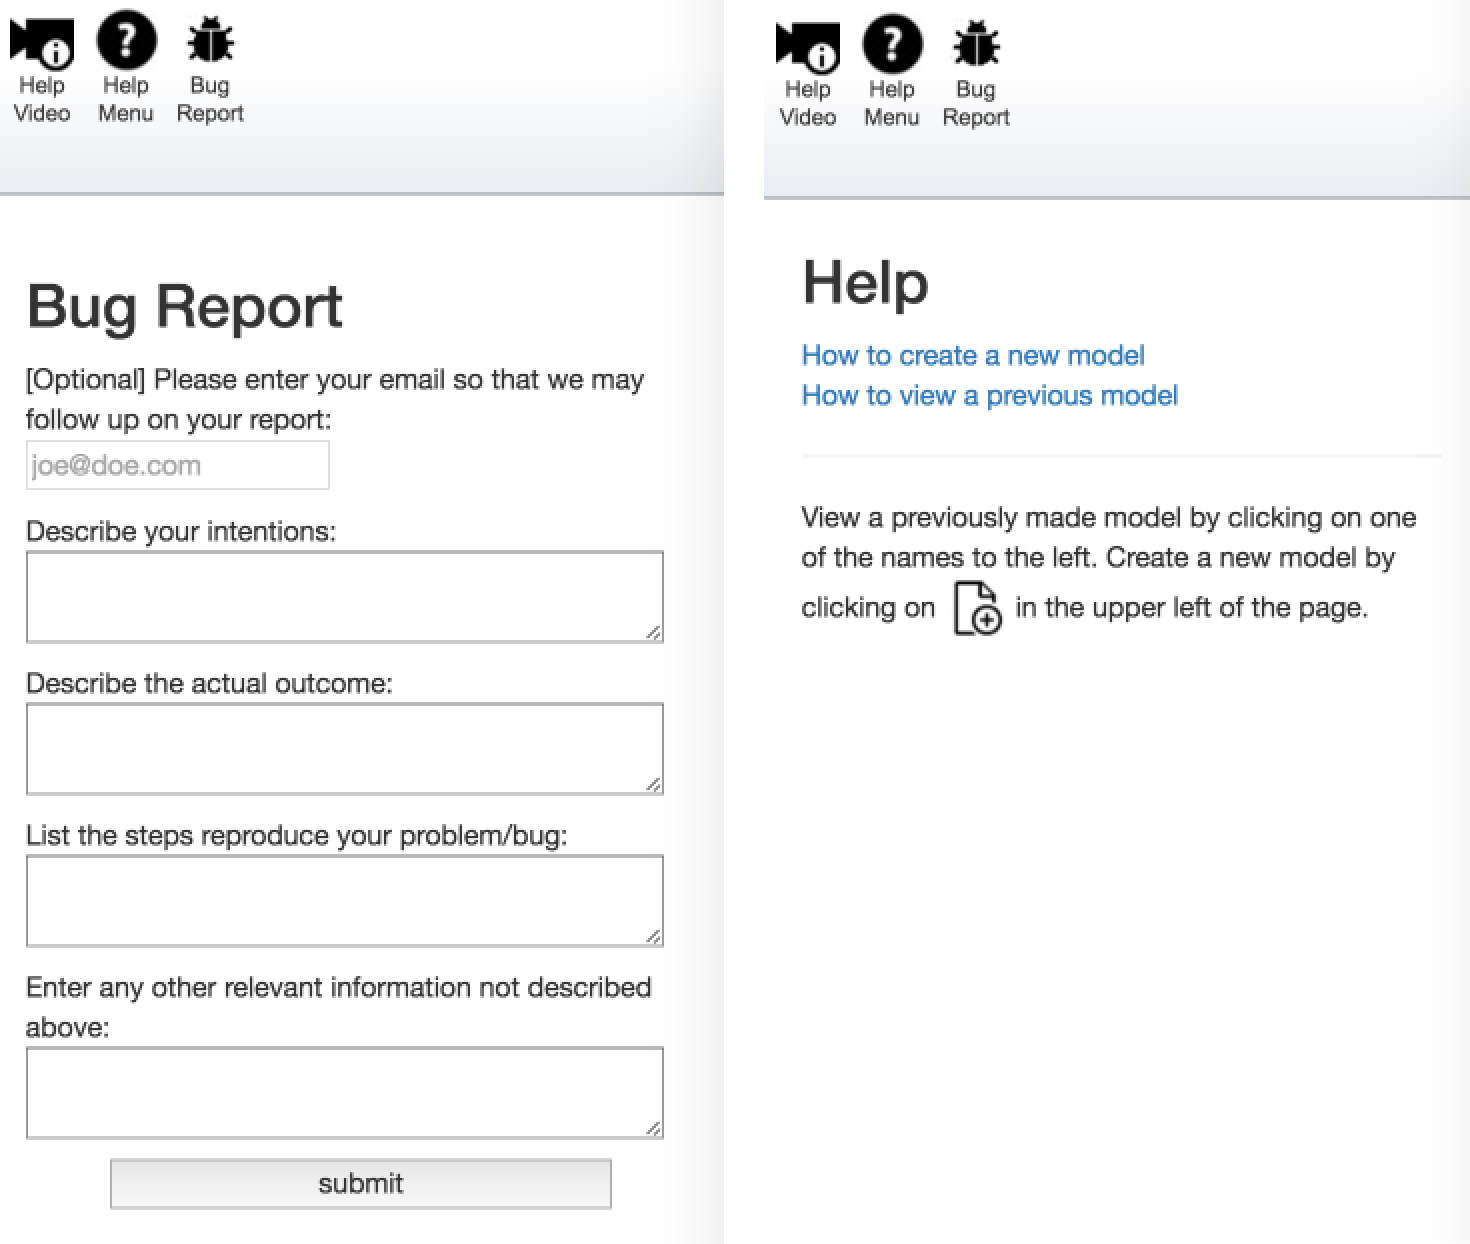
\includegraphics[width=.75\textwidth]{newmenus}
\caption[OASIS bug report and help menu additions]{Left: Bug report submission menu. Right: Help menu with directions based on page.}
\label{fig:newmenus}
\end{figure}

During some initial user tests, users found it difficult to find help on what to do, or how to do something. At the same time, we realized it was difficult to replicate and fix problems described by users in the user feedback section. Our attempt at solving these problems was the implementation of the help and bug report menus. These menus, when selected, would replace the space previous occupied by user feedback. The bug report menu allowed users to submit bug reports to the developers to improve the website. As shown in Figure \ref{fig:newmenus}, information submitted included the intent of the user and methods of reproduction. Using the information acquired, the goal would be improving the quality of the site and reducing the number of bugs users encountered. The help menu included information based on what page the user was browsing, and included animated gifs to display what actions needed to be done.  \\

OASIS is in a state of constant development and improvement, with help from a team of dedicated developers and users. From the enhancements listed in this section, the number of bugs has decreased while the quality of user experience increased. Using the knowledge gained from prior improvements, I applied the same concepts in creating this thesis work. \\

\section{Stroke Recognition}

Since the user's only input into the sketching interface is a series of recorded gestures, some method of interpreting those actions is necessary. Recognizing gestures is difficult because the system needs to recognize that different inputs can often have the same or similar meaning. The amount of variability in a gesture or stroke is sometimes difficult to account for and sometimes the smallest inconsistency can create a wildly different classification. At the same time, the opposite may also be true; an extra action at the end of a gesture may be the defining difference between two classifications. \\

\subsection{Human Input Recognition}
%talk about the difficulty of human input, bring up an example
One example of the difficulty of recognizing human input is reading human handwriting. The variability in each person's style of writing produces a problem where infinitely many inputs may imply the same meaning, as exampled in Figure \ref{fig:handwriting}. According to a survey conducted by Plamondon and Srihari, the inputs to handwriting systems are often separated into two groups: online and offline \cite{handwritingrec}. Online recognition involves user input being captured by a computer interface, as a representation of time, order, and points. For example, the NPen++ online handwriting recognizer collects up to 200 points per second, based on the user's pen input using a Wacom tablet \cite{npen}. Offline recognition refers to a user writing on a physical surface, and that information being scanned and  digitally processed. While online recognition is typically faster and more accurate due to more information being collected \cite{neural2011}, the offline recognition of physical handwriting recognition cannot be ignored, due to its prevalence in everyday life \cite{handwritingrec}. This thesis work uses solely online recognition, as the architectural sketching interface is built on the web for maximum availability to users everywhere.

\begin{figure}[ht]
\centering

\includegraphics[width=.75\textwidth]{catwriting}
\caption[Examples of handwriting variations]{Above is an example of how three writings of the same word, even by the same person, can look different and contain the same meaning.}
\label{fig:handwriting}
\end{figure}

The use of machine learning has been extremely prevalent in human input recognition due to its high accuracy. Many types of machine learning algorithms have been employed to recognize human handwriting, such as hidden Markov models \cite{hmm1994} and neural networks \cite{neural2011}. However, the main drawback of machine learning based approaches is that they all require a large amount of data. In order to learn the finer details between different inputs, a learning algorithm must process a considerable amount of training data before it is effective. For example, the NPen++ recognizer uses a training set of roughly 13,000 words \cite{npen}, while the IAM English sentence database for handwriting recognition contains over 80,000 samples \cite{iamdatabase}. In this work, we choose to take a geometric approach to recognizing user input. While it may be less accurate and less flexible, a geometric approach allows for a faster implementation and tighter control on acceptable input. \\

\subsection{Other Recognizers}

While one recognizer was used most prominently, two other recognizers were also researched. One was a fuzzy recognizer developed by Fonseca and Jorge \cite{fuzzylogic}. This fuzzy logic based recognizer first created strokes (a series of points) and shapes (a recognized stroke), and computed a number of geometric features based on each strokes. Using the features extracted, Fonseca and Jorge created rules, along with allowable percentiles to determine the identity of a stroke. For example, to assist in identifying a circle, they used a \textit{thinness} ratio, which is defined as the perimeter square divided by the area of the convex hull. For different shapes, the allowed values for each of the ratios differed. When a user entered a stroke, the features would be extracted, and ratios calculated. Based on the ratios, a likely candidate could be chosen. Possible classifications included arrows, squares, rectangles, triangles, and circles. \\

While the accuracy of the implementation was high (over 90 percent successfully recognized \cite{fuzzylogic}), and the design was simple to understand and implement, a few factors led me to not pursue this any further. The implementation seemed to require heavy micromanagement of ratios. The implementation did not offer any methods of calculating the cutoffs using training data, leaving me to infer the adjustments were made by hand. While it appeared to work very well on geometric shapes, I had a difficult time recreating the process well on symbols such as letters of the alphabet. The metrics work well on simply defined user input such as as square or triangle, and it worked well on simple letters such as `C` or `T`, but I found it difficult to mathematically define more complex letters such as `B` or `Q`. When creating this application, the initial idea was to classify objects using letters as identifiers. Without a confident method of identifying letters, I felt I could not proceed at the time. Overall the fuzzy logic recognizer was intriguing and promising but did not fit my goals and purposes. \\

Another recognizer researched was a HMM machine learning based recognizer created by Hu \textit{et. al} \cite{hmm1994}. This recognizer used a      `left-to-right` hidden Markov model to score features such as  stroke tangents, translation, rotation, and scaling. A hidden Markov model is a model in which the system being modeled is assumed to be a Markov process with hidden states. A Markov process is one that satisfies the Markov property, which states that all states of the process are based solely on the current state. In this recognizer, each letter is broken down into segments, and recognized afterwards. This implementation describes an approach using \textit{nebulous stroke models}, which they do not define the letters or any features of letters, or how they are segmented. The program itself defines the most natural way of defining a letter. The models are trained using a 3 step process: letter training, linear word training, and lattice word training. Letter training involves training the system on single letters, linear word training uses whole words, and lattice word training transforms all words into finite state networks, and the system is trained on those. \\ 

Overall the hidden Markov model based approach was well defined, but it was overly complicated for my needs. If I had used this approach, a vast majority of my time would have been spent implementing and refining the recognizer into my system instead of developing an interface for OASIS. My primary goal, first and foremost, was to develop a sketch-based interface for OASIS, and not necessarily develop a unique recognizer.

\subsection{\$N Recognizer}
%$N, $1, explain in detail
One recognizer that I tested and used extensively was the \$N recognizer. There existed a few reasons for initially relying heavily on this recognizer for recognizing nearly everything in the system. One, the recognizer was simple to implement and modify. Second, the system was flexible in its ability to recognize both shapes and letters. Lastly, it did not require any training data, so the addition of new recognizable symbols was effortless. \\

The \$N is a lightweight, concise multistroke recognizer that generalizes one multistroke to all possible multistrokes \cite{dollarN}. To understand the \$N recognizer, we must first review its predecessor, the \$1 recognizer for single strokes. The \$1 recognizer is a lightweight, unistroke recognizer that classifies unistrokes based on templates \cite{onedollar}. The \$1 recognizer works in 4 steps: resampling the path, rotate based on indicative angle, scale and translate, and find optimal angle. First, the user drawn stroke is resampled such that the distance between points is equidistant. This necessary to ensure equal comparisons between quickly and slowly drawn strokes. Next, the indicative angle is found, which is defined as the angle between the first point drawn and the centroid of the stroke. This is rotated to zero degrees and helps normalize all strokes to a common angle. After rotating, the stroke is non-uniformly scaled to a reference square. This allows the recognizer to directly compare the user drawn stroke to the templates, and assume that changes in distance are due to rotation and not aspect ratios. After the scaling of the stroke, it is translated to a reference point, usually the centroid at (0,0). The above steps are also applied to all the template to ensure each point in the stroke matches to one point in each of the templates. Finally, to find the optimal angle, the stroke is scored against all templates, and the stroke with minimal differences is determined to be the classification for the stroke. \\

\begin{figure}[ht]
\centering
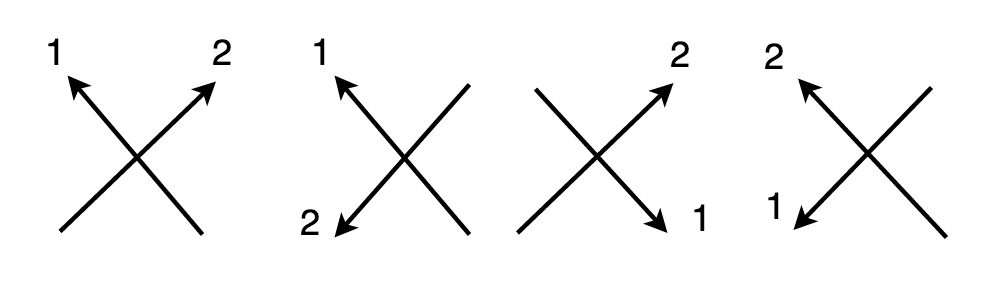
\includegraphics[width=\textwidth]{dollarnstrokes}
\caption[Examples of stroke permutations]{Some permutations possible for an 'X'. The numbers represent the order in which they are drawn, and the arrow represents the direction of the stroke.}
\label{fig:nstrokes}
\end{figure}

The \$N uses the same processes as the \$1, except on multiple strokes. The main challenge of multistrokes is that any of the strokes can be drawn in any order and from any direction. As shown in Figure \ref{fig:nstrokes}, even a simple two stroke gesture has multiple combinations. The \$N recognizer orders the points in each possible permutation - essentially treating each multistroke permutation as a unistroke. A Heap Permute is used to generate all possible permutations of strokes \cite{dollarN}. The \$N also operates with bounded rotational invariance, meaning an object flipped completely upside down (rotated 180 degrees) will be recognized as a completely different gesture. The bounds for rotation are set to $\pm$ 90 $^{\circ}$.  These permutations are generated for each template, then compared to the user input. The one with the lowest score (smallest difference) is chosen as the classification for the user input. \\

During the initial development of this work, I relied heavily on the \$N recognizer to recognize all objects in the system. However, it failed to accurately classify different combinations of strokes too often. The exhaustion of all permutations of combinations of strokes meant that it more often than not found connections between combinations of strokes the user did not intend. While it may have been possible to more intelligently select combinations of strokes to classify, it became apparent that this tool was far too flexible for our needs. In chapter 3, we will discuss our replacement solution for this recognizer and how we overcame these issues.

\section{Related Software}

This work shares qualities and goals with other sketching software. Two such examples are Lightsketch created by Glaser \textit{et. al} \cite{glaser2003sketch} and Yi-Luen Do's VRSketchpad \cite{do2001vr}, both of which are also architectural sketching interfaces. LightSketch is similar to OASIS and uses sketching vocabulary \cite{glaser2003sketch} similar to the new sketching interface. In particular, LightSketch also shares a `sketch-based` interface with a minimal user interface. Similar to this sketching interface, LightSketch can also recognize shapes shapes and symbols. However, Lightsketch does not have any shape indications or overlaid shapes to indicate to the user the interface's intent. Also, LightSketch does not appear to have any methods of editing previously drawn primitives, while this sketching interface allows users to change, edit and reclassify previously created lines. \\

VRSketchpad also employs a freehand sketch approach to their interface. Similar to our implementation, VRSketchpad processes the user design and translates the drawings into 3D objects. VRSketchpad also has multiple levels to processing to create shapes, irregular shapes, and pieces of furniture. However, VRSketchpad contains a much busier interface than our own, which is devoid of buttons and modes. Unlike our implementation, VRSketchpad has no recognition before processing the drawing into a 3D model. Therefore, we can give the user a better idea of our interpretation of his/her design before creating the 3D model.\\

% Rubine's specifying gestures by example
% SATIN
One example of a non-architectural sketching interface is the Gesture Recognizers Automated in a Novel Direct Manipulation Architecture (GRANDMA) created by Rubine. Rubine describes a series of features that are incrementally computable in constant time per input \cite{rubinegestures}. These features include cosine and sin of the initial angle of the stroke, duration of the strokes, bound box diagonal of the stroke, and distance of the stroke in total. These features are also used in other applications, such as SATIN, a toolkit for informal ink-based applications \cite{satin}. In order to classify strokes, weights were attached to features depending on their importance to that classification. Rubine's system also had the ability to reject classification if the gesture was deemed ambiguous or if it was not confident in its recognition. When a user created stroke was run against a template, the highest scoring classification would be applied. These features were applied to create his gesture-based drawing program (GDP). GDP was a simple drawing program with robust features by drawing unistroke commands to specify certain actions. For example, a user could use the `delete` command, and the next unistroke would be executed as a delete command. Our implementation uses a similar system when attempting to classify rectangles. Also, both interfaces use a minimal interface, relying solely on user drawn strokes. However, Rubine's implementation uses a training set to learn the unistrokes recognized by the program, while my implementation does not require the use of any training data. In chapter 4, we will discuss further in depth the features chosen to represent our objects. \\

\section{Summary}
This chapter provides an overview of the works that influenced the design and development of this project. The previous feature development on the OASIS system helped to develop an interface suitable for OASIS itself. As we will discuss in chapter 3, many of the technologies used in OASIS will also be used to develop this work. Different works in human input recognition led me to choose a geometric based approach to classifying user strokes. This work will provide an enhanced user experience when designing models on OASIS.
    %%%%%%%%%%%%%%%%%%%%%%%%%%%%%%%%%%%%%%%%%%%%%%%%%%%%%%%%%%%%%%%%%%%
%                                                                 %
%                            CHAPTER THREE                          %
%                                                                 %
%%%%%%%%%%%%%%%%%%%%%%%%%%%%%%%%%%%%%%%%%%%%%%%%%%%%%%%%%%%%%%%%%%%
\chapter{System Overview} \label{sec:system}

As stated in chapter 2, this thesis is an extension and modification of OASIS. The previous iteration of the user interface employed a 'drag-and-drop' method of introducing new elements. This chapter will explain in detail the processing entailed before recognizing the user's input. First, I will discuss where and how this work modifies the OASIS pipeline. The next section contains a detailed overview of strokes, the processing of those strokes, and extraction of useful metrics from them. Next, we cover actions available to the user in the sketching interface, such as creating walls, windows, and deleting previous objects. The final section consists of implementation elements, and its similarities and differences compared to OASIS.

\section{OASIS Pipeline}
In order to understand where this work improves OASIS, first I must discuss the pipeline OASIS follows to create new models. Figure \ref{fig:oasispipeline} illustrates the steps to completion from a user design to a finalized rendering. First, a user sketches a top-down 2D design of a room using the sketching interface. Users can then drag and drop walls, windows, and furniture onto a canvas. The placements and angles of furniture, the cardinal direction of the room, as well as its location in the world may be edited. Afterwards, the objects are converted into a primitives file which is interpreted by the physical sketch interpretation algorithm. This primitives file contains data about the attributes of walls and furniture, as well as room configurations. The physical sketch interpretation algorithm automatically interprets the sketch and exports it as a watertight triangle mesh  \cite{cutler2009inferring}. This mesh is rendered without lighting effects and simply confirms that the user's intentions were adequately interpreted into 3D from their 2D sketch. From any of their created meshes, users may create a simulation on the task manager page. Tasks may be edited with dates, times of day, timezones, and weather effects. After receiving a user-configured task, our server creates image textures based on the attributes set by the user. These textures are then used to map onto a finalized rendering shown to the user. \\

\begin{figure}[ht]
\centering
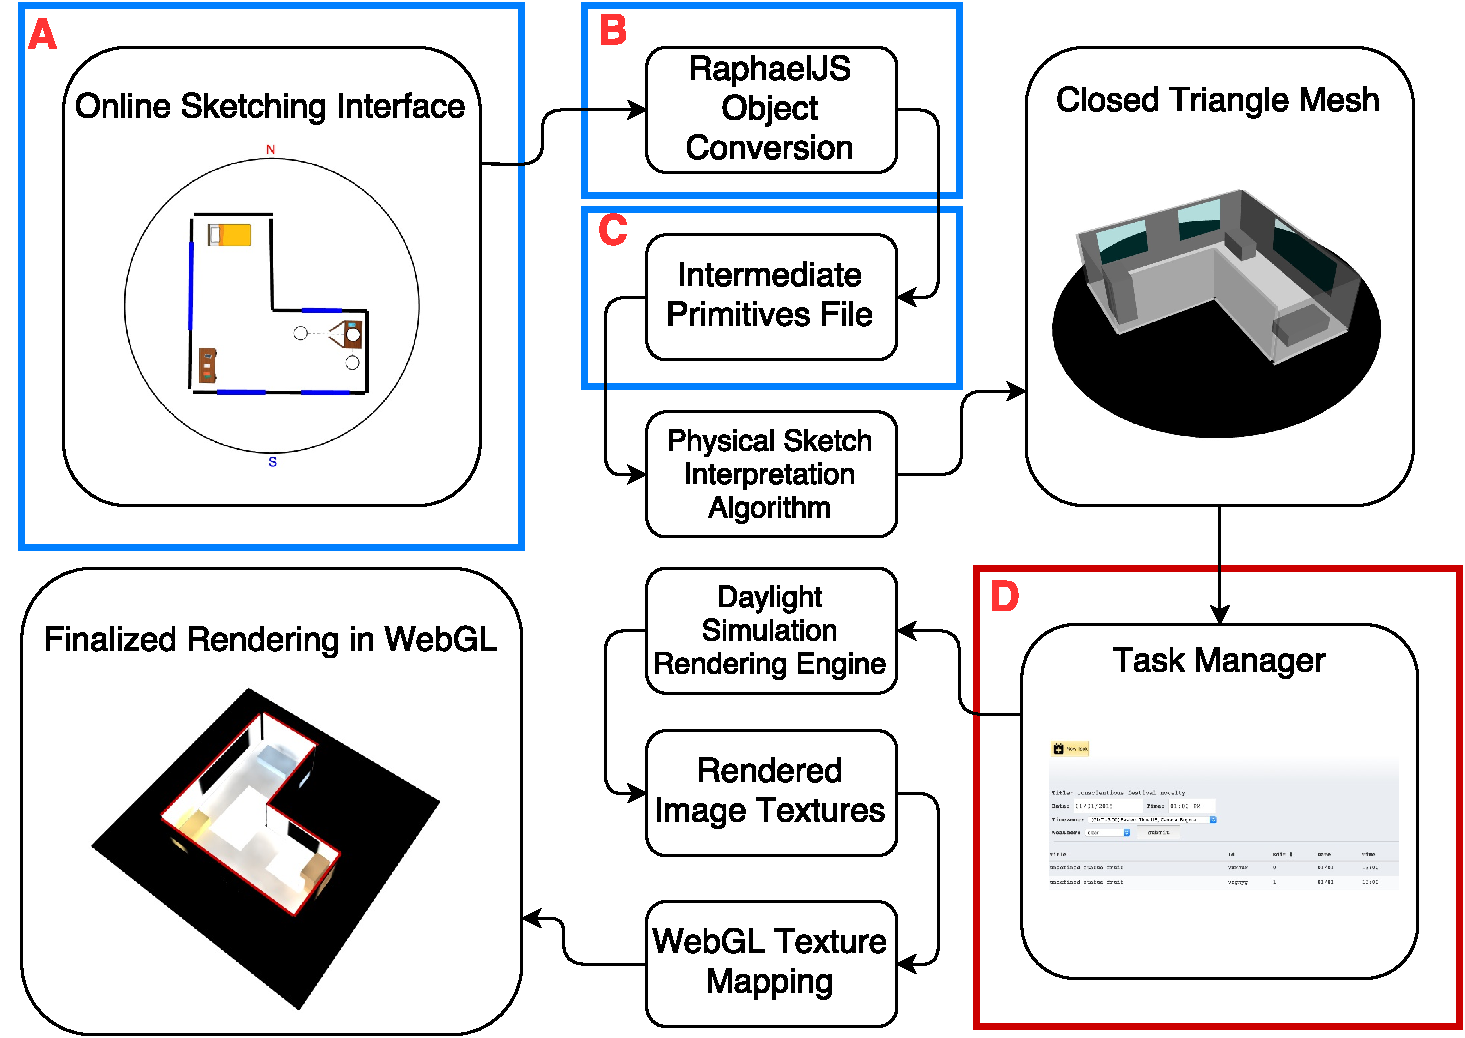
\includegraphics[width=\textwidth]{OASISpipeline2}
\caption[OASIS pipeline diagram]{Above is a diagram of the OASIS pipeline. Author's primary contributions are boxed in blue. Previous work is boxed in red.}
\label{fig:oasispipeline}
\end{figure}

In Figure \ref{fig:oasispipeline}, the boxes highlight which areas of OASIS I directly contributed to. The main contributions of this thesis to OASIS are the improvements to the online sketching interface, the RaphaelJS object conversion, and the modification of the intermediate primitives file. \\

\section{System Pipeline}
The system pipeline illustrated in Figure \ref{fig:systempipeline} outlines the primary stages of this thesis. Comparing to Figure \ref{fig:oasispipeline}, Figure \ref{fig:systempipeline} would belong between Figure \ref{fig:systempipeline}A and B, as shown in Figure \ref{fig:middlepipeline}. Improvements are also made to both the sketching interface and object conversion pipeline steps, which will both be discussed later in this chapter.

\begin{figure}[ht]
\centering
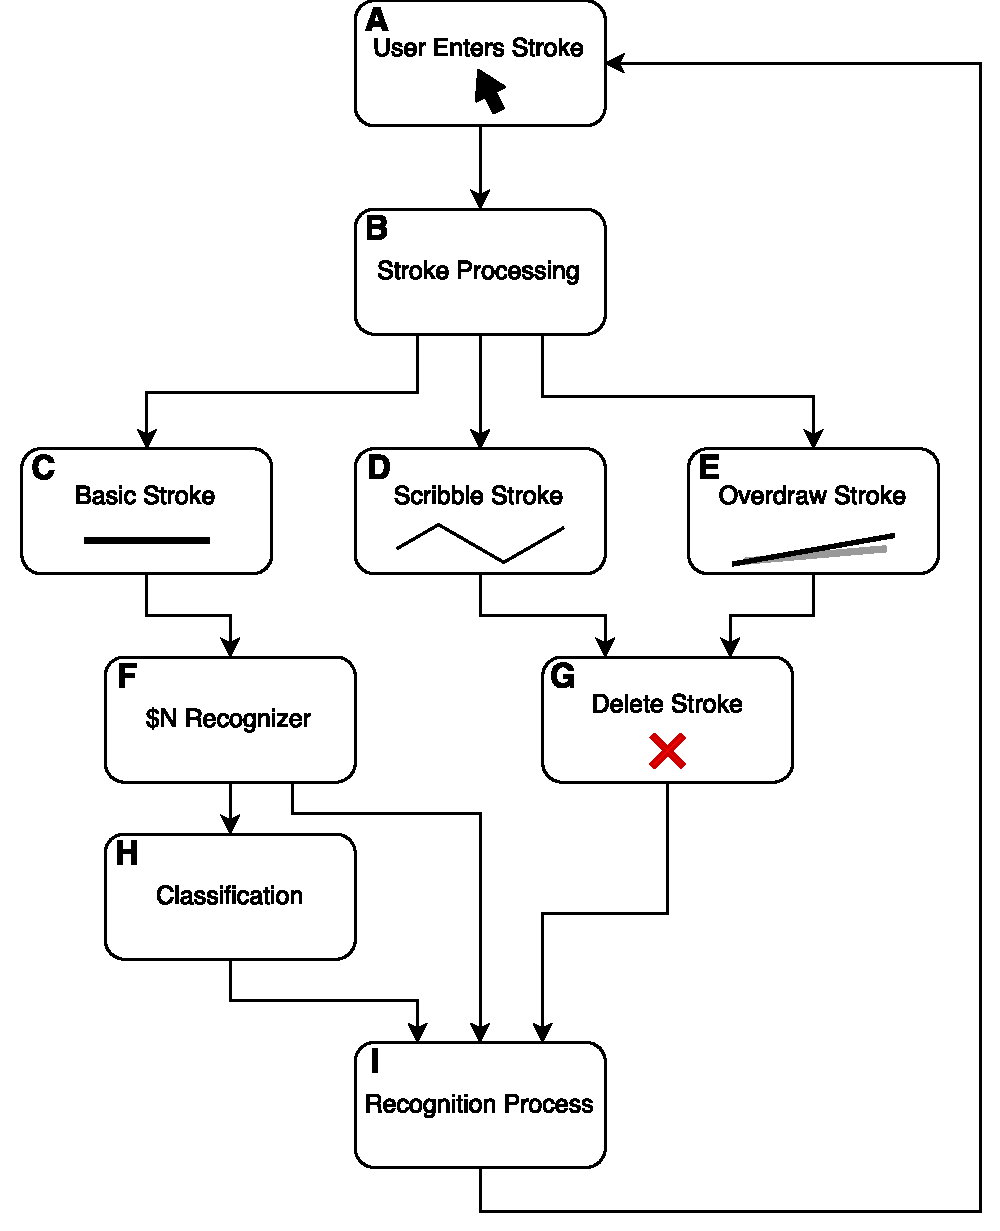
\includegraphics[width=.75\textwidth]{pipeline}
\caption[Sketching interface system pipeline diagram]{Above is a diagram of the system pipeline. This pipeline is contained within the stage represented by \ref{fig:middlepipeline}-A}
\label{fig:systempipeline}
\end{figure}

First, the system accepts a stroke, processes them into a standardized form, and create new attributes about the stroke. These steps are necessary to ensure accuracy when comparing different strokes. Afterwards, we identify the type of stroke based on properties calculated in the previous step. If the stroke is determined to be a scribble or overdraw, the system compares it against other strokes to determine if a deletion is necessary. If not, it is treated as a normal line segment or wall, and the system proceeds onto the recognition phase.  \\

\begin{figure}[ht]
\centering
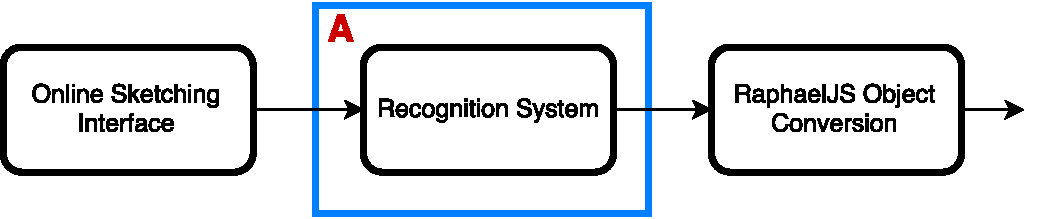
\includegraphics[width=\textwidth]{middle}
\caption[System pipeline diagram]{Above is the placement within the OASIS pipeline of the recognition system in which a majority of this work is contained.}
\label{fig:middlepipeline}
\end{figure}

If the stroke is determined to be a basic stroke after processing, it is fed into a the \$N recognizer to check if it similar to one of the template letters. If so, it will be used to reclassify an object according to the letter drawn. If not, it is treated as a normal line segment or wall and continues to the recognition phase. In the recognition phase, the system reevaluates the context of the set of strokes it has been given. The system will recognize any objects, fit an appropriate shape to them, display it to the user, and classify it under an object template.

\section{Stroke Processing}
\label{sec:strokeproc}

A point is defined as single pair of x and y coordinates. A stroke is a series of points on a canvas, and is the one of the most basic foundation data types in this system. To create a stroke, the user simply clicks anywhere on the interface, and moves their mouse to any other point on the interface without moving outside the boundaries. The system automatically records coordinates every time the mouse moves, creating a sequence of points. When the user releases his/her click, the points are converted into a stroke. In this section, I will review the processing done to these to simple points to interpret the user's intent.

\subsection{Stroke Resampling}
\label{sec:resample}

\begin{algorithm}
\caption[Pseudocode for resampling]{Psuedocode detailing resampling of a stroke}
\label{alg:resampling}
\begin{algorithmic}[1]
\Function{Resample}{points, numPoints, numDivisions}
\State $i \gets  PathLength(points) / (numDivisions -1)$
\State $d \gets $ 0
\State $resampled \gets $ [ ]
\For{$i = 0 \to numPoints$ }
    \State $m \gets  distance(point_{i-1}, point_i)$
    \If{$d+m < i$}
        \State $px \gets point_{i-1}.x + ((i-d)/m * (points_i.x - points_{i-1}.x))$ 
        \State $py \gets point_{i-1}.y + ((i-d)/m * (points_i.y - points_{i-1}.y))$ 
        \State $resampled \gets (px, py)$
        \State \textbf{insert} $(px,py)$ \textbf{in} points \textbf{at} i
    \Else
        \State $d = d+m$
    \EndIf
\EndFor
\State \textbf{return} $resampled$
\EndFunction
\end{algorithmic}
\end{algorithm}

After recording the raw coordinates of a stroke from the user, the first process required is resampling the stroke. Since a stroke is list of x and y coordinates, it is actually a series of short line segmenets. Unfortunately, due to differences in computer processing and human drawing speeds, these line segments may vary in length. The main purposes of resampling are to eliminate the inequality created by differences in speed when drawing strokes, and to remove clumping of points commonly created around corners. The inequality of the spacing between points of the line affects the scoring algorithms that rely on weighting metrics between all points equally. Algorithm \ref{alg:resampling} outlines the process to resample any number of points to \emph{numDivision} number of points. The algorithm finds the appropriate number of points, and the distance between each one such that they are all equidistant to their neighbors. There must a point every \emph{distance} length away, so we follow the stroke's path , point by point, creating a new point every time that threshold is crossed. At the end, there will exist exactly the number of points specified with equal distances between them. There is one flaw to this algorithm: it creates points that were not drawn by the user, and therefore the new set of points may not truly represent the user's original line. However, if the number of divisions is sufficiently high enough, the newly created set of points is a good approximation of the initial stroke. The average number of points per 150 pixels is approximately 30, and after resampling is the \emph{numDivision} number of points. I currently use 24 points per 150 pixels, through usage of the program I have found that using this number both generally lowers the number of points, and keeps a high degree of similarity to the user's original sketch.\\

Another possible method of resampling the line is to fit curvature of the line better. To accomplish this, extraneous points are removed from straight edges, and points are added to better define edges and curves. While this creates a better fitting line to the user's original input, the main purpose of fitting a line to the curvature is to lower the total number of points while retaining the shape of the line. However, my primary purpose of resampling the lines is to retain accuracy of our scoring algorithms by ensuring each point will have equal influence over the scoring of strokes or shapes.

\subsection{Line of Best Fit}
\label{sec:bestfit}
Since strokes contain many data points, it becomes very costly and difficult to draw comparisons between them. In cases where the strokes are perfectly straight lines, stroke comparison is simple. Properties such as angles and intersections between two or more lines are straightforward to calculate. Since not all strokes created are straight lines, it can be difficult to measure such attributes. In order to compare strokes, I have chosen to compute a linear line of best fit to generalize properties about a stroke. This reduces all strokes to straight lines, simplifying the process of comparing them. Treating the points of a stroke as scatter plot, a line of best fit will describe a set of properties that best fit the stroke. These properties include the slope, y-intercept, and the $r^2$ value. The slope determines the steepness of the line of best fit, the y-intercept controls the translation of that line, and the $r^2$ value represents how well the line fits the stroke's points. I used a least squares method to find my line for best fit, identifying the line with the least squared difference between it and each of the points in the stroke.

\subsection{LengthRatio}
\label{sec:lengthratio}
%definition of a stroke
%resampling
%length ratio, scribble

An important metric of a stroke is the line length to path length, or the \textit{LengthRatio}. The line length is the Euclidean distance from the first point to the last point. The path length is the summation of every line segment contained within the stroke. One useage of this metric is to determine if a user has drawn a line sufficiently close enough to a straight line. Since it is incredibly difficult to draw a perfectly straight line, I recognize when a user's stroke is close enough to a straight line, and fix it accordingly, as shown in Figure \ref{fig:walls}B-C. The equations for the calculation of the \textit{LengthRatio} are described below.

\begin{equation}
\label{equ:ratio1}
LineLength = distance(point_{0}, point_{n})
\end{equation}

\begin{equation}
\label{equ:ratio2}
PathLength = \sum_{i=0}^{n-1} distance(point_{i}, point_{i+1})
\end{equation}

\begin{equation}
\label{equ:ratio3}
LengthRatio = \dfrac{LineLength}{PathLength}
\end{equation}

Essentially, as the \textit{LengthRatio} approaches 1, the closer a stroke is to a perfectly straight line. Through some basic testing, I've determined .95 to be a reasonable cutoff for fixing crooked paths. \\

The same ratio is also used to determine strokes that are not definitely not straight lines, or `scribbles`. Scribbles are lines that are haphazard and random. To detect a scribble, the \textit{LengthRatio} is used, but with a different cutoff. The minimum \textit{LengthRatio} to be a line is .7, and any strokes under that are determined to be scribbles. 

% A very similar ratio is also used to determine strokes that are not definitely not straight lines, or `scribbles`. Scribbles are lines that are too haphazard and random. To detect a scribble, a \textit{AverageLengthRatio} is calculated every \emph{m} points, and averaged, as shown in Equation \ref{equ:ratio4}. A scribble typically has abrupt changes in direction, leading to a very high average \textit{LengthRatio}. An \textit{AverageLengthRatio} is used instead of an overall \textit{LengthRatio} in order to avoid capturing strokes such as a curve, which has a relatively high \textit{LengthRatio} compared to a straight line but a low \textit{AverageLengthRatio} compared to a scribble. The purpose of recognizing a straight line from a scribble is to delete previous strokes, which will be detailed further in the next section.

\section{Sketching Interface Actions}

In this section, we will discuss the features and actions available to the user to create and edit their designs. Since one goal was to preserve the simplicity of drawing, not many extraneous buttons or menu options were added. I did not want the user to feel pressured to remember hotkey combinations or highly specialized methods to perform certain actions. At minimum, the proposed new sketching interface has all the features of the previous system, plus added flexibility and ease of use.

\subsection{Walls and Windows}

As described earlier in Section \ref{sec:strokeproc}, a stroke is created on the new interface by clicking on the interface and dragging to another location. An example of how a user would create a wall is outlined in Figure \ref{fig:walls}A-C. At a base level, all strokes are considered walls until recognized or classified as otherwise. The next chapter will cover the classification and recognition of objects in further detail.

\begin{figure}[ht]
\centering
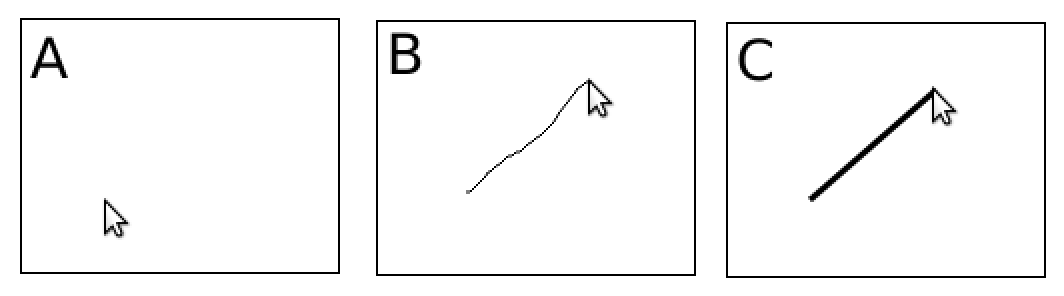
\includegraphics[width=\textwidth]{walls}
\caption[How to create a wall using the sketching interface]{How to create a wall using the sketching interface.}
\label{fig:walls}
\end{figure}

The new sketching interface mimics how one would draw with pencil and paper, without the need to click on buttons or referring to toolbar. As demonstrated in Figure \ref{fig:walls}, the strokes will snap to a straight line if the LengthRatio has crossed a threshold of .95. This is achieved by replacing the previously recorded points with a segement of the line of best fit. This is determined by finding the points on the line of best closest to the first and last point created by the user. Given that most physical walls are straight, and that it would be difficult to straighten lines without any tools on the interface, it made sense to automatically fix slightly crooked walls. Overall, it was a change that resulted in much cleaner looking designs. \\

Windows can be created just as seamlessly as walls in the new interface. Windows must be attached to a wall, and cannot be longer than the wall it belongs to. As shown in Figure \ref{fig:windows}-A, a user mouses over a wall, changing the wall's color to red. Next, the user clicks on the wall and drags the wall to the desired length, as illustrated in Figure \ref{fig:windows}-B. Finally, to create the window, the user releases his or her mouse click, snapping the window to the wall, as depicted by Figure \ref{fig:windows}-C.

\begin{figure}[ht]
\centering
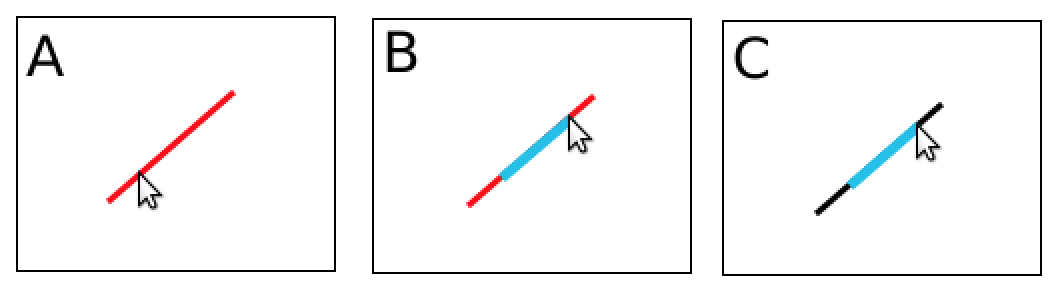
\includegraphics[width=\textwidth]{windows}
\caption[How to create a window using the sketching interface]{How to create a window using the sketching interface.}
\label{fig:windows}
\end{figure}

The window snapping algorithm uses the best fit line of the wall it is attached to. The user chooses the length of the window by designating a start and end point, and the the slope of the window is determined by the slope of the line it is attached to. In order to allow for flexibility, walls do not need to be dragged in the exact direction or orientation to snap to the wall. The proposed window can be dragged into any angle, and even beyond the length of the wall. However, should a user mistakenly enter the window creation process, he/she can drag the cursor such that it creates a perpendicular angle with the wall, ensuring that the window does not get created at all. Regardless of how long the wall is dragged, it will always snap up to a maximum of 5 percent away from the end, towards the center of the wall. This is to allow some space for the window, and to avoid some bugs that have been discovered with windows attached walls that are equally as long.

\subsection{Deleting Strokes}

Should the user make the inevitable mistake, the ability to delete strokes would be a welcomed feature. Keeping in the spirit of design without using a toolbar, users can 'scribble' or draw over their previous strokes to delete or modify them. The act of modifying a stroke is very similar to the previously described actions. \\

It is simple to scribble out a previously drawn stroke. As shown in Figure \ref{fig:scribble}, a user find the stroke he/she wants to remove, then sketches a random stroke resembling a scribble over the chosen stroke, and both strokes disappear.

\begin{figure}[ht]
\centering
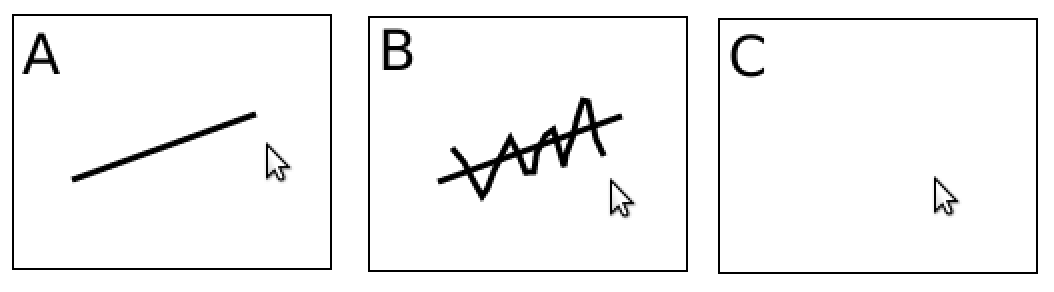
\includegraphics[width=\textwidth]{scribble}
\caption[How to delete a stroke by scribbling]{How to delete a stroke by scribbling.}
\label{fig:scribble}
\end{figure}

As mentioned before in Section \ref{sec:lengthratio}, if the LengthRatio is under .7, a stroke is classified as a scribble. If a stroke is detected as a scribble, we search for strokes whose points are near those of the scribble. If another stroke is in the immediate area, then both strokes are removed from the sketch. However, the strokes do continue to remain in the system, allowing for the possibility of an undo feature in the future.\\

To draw over a stroke, a similar process to scribbling is employed. First, the user finds a stroke he/she would like removed, as exhibited in Figure \ref{fig:scribble}. The stroke is currently only greyed out in the image and not the application itself. However, it could be a feature for development in the future, since the viewing of previous strokes may visually assist the user when designing. Next, the user draws a line with similar angle, length, and positioning to the undesired stroke. Finally, the previous stroke is removed and the new stroke remains.

\begin{figure}[ht]
\centering
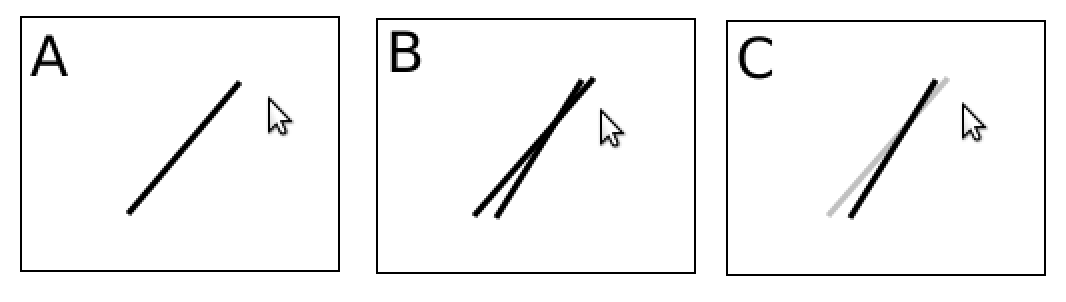
\includegraphics[width=\textwidth]{overdraw}
\caption[How to overdraw a previous stroke]{How to draw over a previous stroke. The removed stroke is greyed out only for this figure, to help visualize the removal.}
\label{fig:overdraw}
\end{figure}

The process behind overdrawing a stroke is also similar to that of scribbling. However, instead of checking for the presence of a scribble, I check for the distance between the overdraw stroke and every other stroke. The distance between strokes is calculated between the centers of the strokes. We compare the stroke's properties taken from its line of best fit to its closest neighbors, which are only strokes whose centers are within half its \textit{pathLength} away from its own center. If any other strokes are similar enough in length and angle, we delete the previous stroke and allow the newly drawn stroke to remain. If no strokes fit the criteria, then the stroke is treated as a normal wall. \\

Previously, a two dimensional grid was used to store stroke information and compare location data. While it is more computationally efficient with extremely high numbers of strokes, the overhead and complexity to maintain such a data structure with low numbers of strokes far outweighed the benefits. After testing with moderately complex models with 20-40 strokes, it was determined that the use of a spatial data structure was either the same or slower speed than checking against all other strokes. Should models become more complex in the future, this data structure could be revisited. However, in its current iteration, there is not enough data in an average model to warrant the use of a spatial structure.

\subsection{Cardinal Direction}

With the production of a new sketching interface, it was necessary to consider a new method of indicating the cardinal direction, such as north or south. The previous implementation was a movable ring surrounding the design area. However, ring would be an inefficient use of space with a rectangular sketching area. The proposed idea is a small north arrow on the canvas indicating the direction of north. The arrow will rotate away from the center every time it is adjusted. Users will be able to easily move the indicator without clicking on a toolbar. The equation used to calculate the angle away from the center given a point and a center is shown in Equation \ref{equ:anglecenternorth}.

\begin{equation}
\label{equ:anglecenternorth}
Angle = \tan{(\dfrac{point_y - center_y}{point_x - center_x})}
\end{equation}

\begin{figure}[ht]
\centering
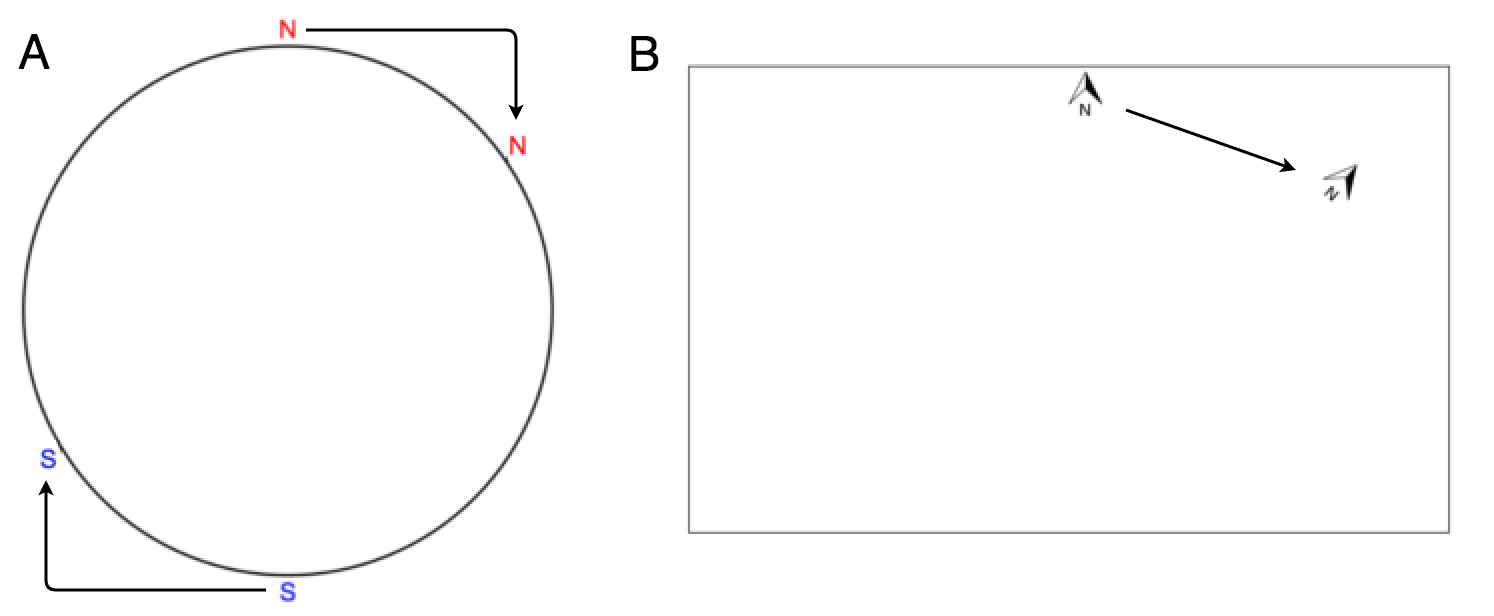
\includegraphics[width=\textwidth]{compass}
\caption[Comparison of cardinal direction changes between interfaces]{An illustration between the two methods of changing cardinal direction in each interface.}
\label{fig:compass}
\end{figure}

\section{System Design and Implementation Details}

In this section, I will give a brief overview of system design choices that are not a direct part of the sketching interface itself. While they do not necessarily directly affect the user, it is important to understand these design choices and their impacts on the user and the future of OASIS.

\subsection{Intermediate Primitives File}

Due to the possible additional complexity of walls, a decision was made to move away from the previous primitives file format. The previous format was designed to recognize physical objects placed on a table, with small numbers of primitives, and record data such as position and orientation. However, in the new interface, with walls and strokes capable of containing over 100 points (and thus over 100 wall segments), the amount of data stored needed to be simpler to store and access. The new proposed intermediate primitives file format will be in Javascript Object Notation (JSON). JSON is a language independent, lightweight, data-interchange format that is easy for humans to read and widely generated and parsed by many operating systems and applications \cite{json}. JSON is often used to transmit data from servers to applications and consists of attribute/value pairs. Given its widespread use, it would allow the data collected in this application more accessible to other programs and make integration with future features simpler. Also, being a standardized format will require less specialized knowledge to understand. Moving forward, the switch to the JSON file format will make the application more accessible for feature development and more manageable to maintain. 

% \subsection{Inclusion of both sketching interfaces}

% Currently, when a user creates a new model, the user has an option to design with either the previous user interface or the new sketching interface. An image of the menu is displayed in Figure \ref{fig:choice}.

% \begin{figure}[ht]
% \centering
% 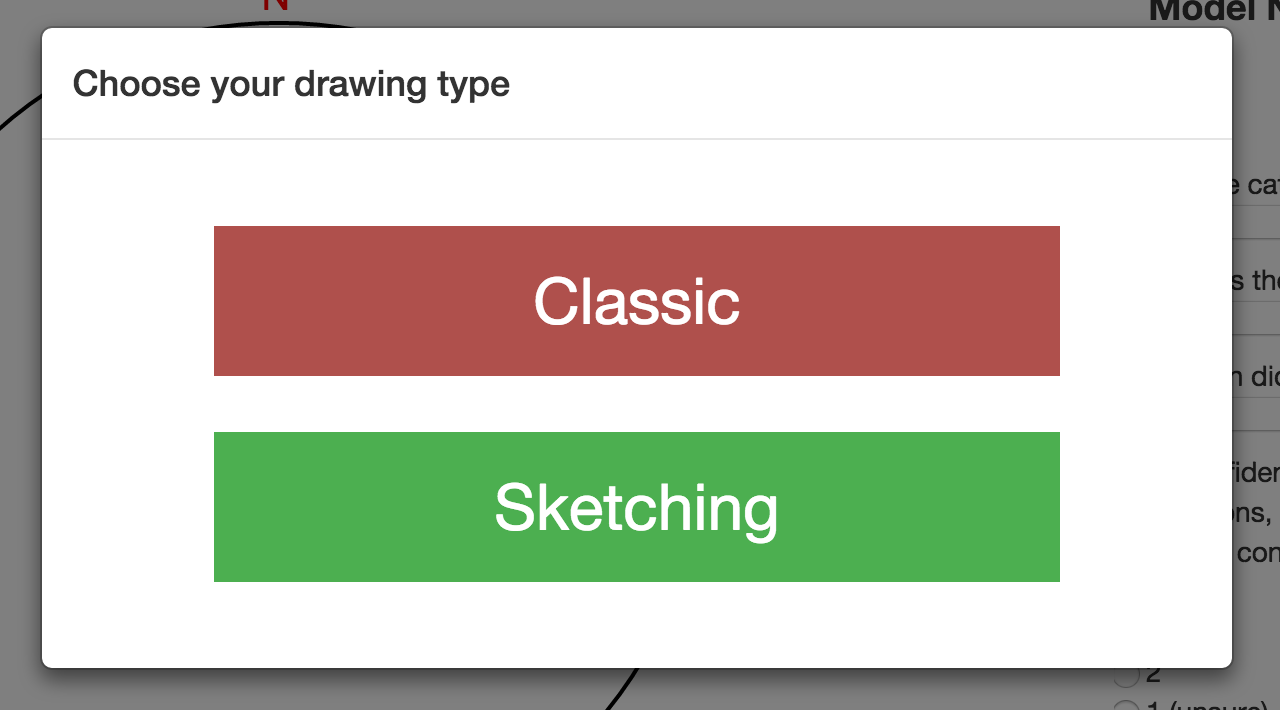
\includegraphics[width=.75\textwidth]{choice}
% \caption[Image of choice between interfaces]{Upon choosing to design a new model, the user may choose between the previous interface or the new one.}
% \label{fig:choice}
% \end{figure}

% The reasoning behind the choice to allow the user to choose his/her method of sketching was to support the decision of the user of the more comfortable interface. While I would be delighted if every single user thought this new sketching interface was undeniably better than the previous one, it is unlikely to true. In a topic as arbitrary as design methodology, every user has his/her unique preferences, and it is not possible to be perfect in every scenario. I believe that it is in the application's best interest to allow each user to select his or her preference.

\subsection{Technologies}

Being an extension and modification of OASIS, it is logical that the two have technologies and frameworks in common. Both applications are built primarily on Javascript, and both rely heavily on the RapahelJS \cite{raphaeljs} framework. RaphaelJS is a vector graphics Javascript framework that supports most major web browsers. RaphaelJS is used to create all the sketching elements, including walls, windows, and furniture. It allowed for the easy creation and manipulation of lines and shapes created by the user. FreeTransform \cite{freetransform}, which is an extension of RaphaelJS, is used for the rearrangement of objects in the sketching interface. Due to the method of storing positional values by RaphaelJS, moving an object multiple times is complex. Both RaphaelJS and its extension, FreeTransform were instrumental in the development of this work.

%talk about the new wallfile
%talk about choice of sketching
%technologies used

\section{Chapter Summary}

This chapter reviewed the pipeline of OASIS and where  this work contributed within that process. An overview of strokes, processing of those strokes, and stroke metrics were provided. Next, I presented the elements and actions available within the sketching interface itself. Afterwards, I discussed some of the design choices behind the development of this thesis and its impact on the application. The next chapter examines in further detail the logic behind recognition and classification of objects in the sketching interface.
    %%%%%%%%%%%%%%%%%%%%%%%%%%%%%%%%%%%%%%%%%%%%%%%%%%%%%%%%%%%%%%%%%%%
%                                                                 %
%                            CHAPTER FOUR                          %
%                                                                 %
%%%%%%%%%%%%%%%%%%%%%%%%%%%%%%%%%%%%%%%%%%%%%%%%%%%%%%%%%%%%%%%%%%%
\chapter{Recognition} \label{sec:recognition}
This chapter reviews in detail the primary contributions of this thesis: the recognition, fitting, and classification of objects in the new sketching interface. The recognition of objects refers to the system's awareness to the presence of a series of strokes representing an object. Object fitting results in a generated shape that accurately represents an object recognized by the system. Lastly, the classification of an object results in the designation of certain attributes determined by its physical properties. These application features use and build from the metrics described in chapter 3.  These components elevate the sketching interface beyond a simple painting program. The system is intended to recognize the input, understand the user's intentions and reiterate that to the user an image that is meaningful and easy to understand. \\

\begin{figure}[ht]
\centering
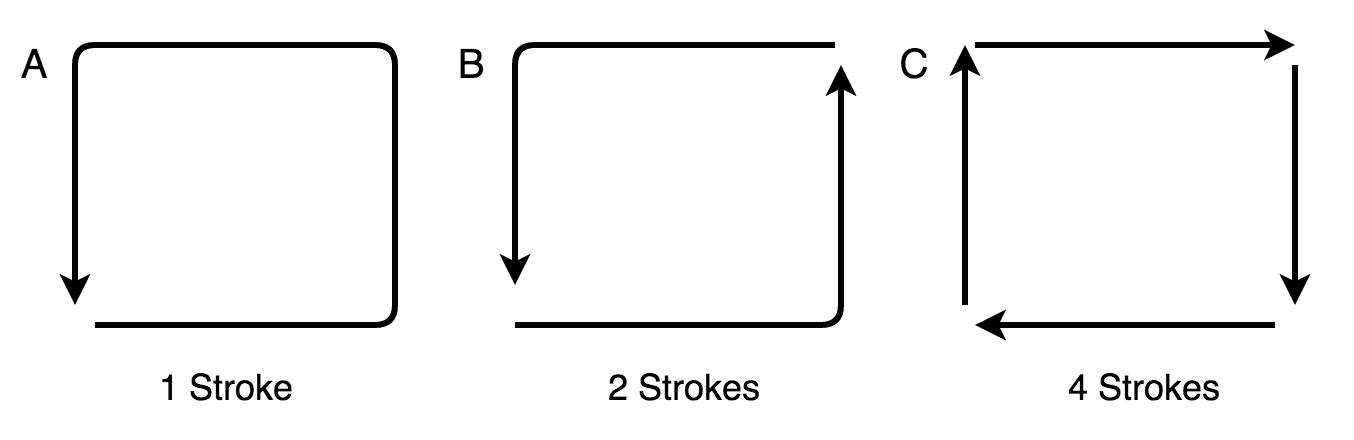
\includegraphics[width=\textwidth]{multistrokes}
\caption[Comparisons between methods of drawing a rectangle using different amounts of lines.]{Illustrated are methods of drawing a rectangle using different amounts of lines. This application currently only recognizes rectangles drawn with four strokes.}
\label{fig:multistrokes}
\end{figure}

Due to the shapes of objects we currently allow in OASIS, all objects may be accurately represented in 2D as a rectangle. Therefore, the algorithms presented are specialized to solve for the subset of shapes similar to rectangles. The problem set is further simplified to recognize only sets of straight lines that are of size 4. However, proposed methods to overcome this limitation will be presented. \\

I present a geometric based approach to recognizing rectangles from user drawn lines. The basic features of a rectangle were analyzed to create metrics useful in determining the existence of a user drawn rectangle. Since multiple rectangles may be created from a common set of strokes, scoring functions are necessary in determining the optimal outcome. Algorithms and analysis for primary scoring functions are displayed and evaluated. Afterwards, in section \ref{sec:classification}, I present a method to classify rectangles based on their attributes. Finally, we will discuss my approach to fit a rectangle to a set of user drawn strokes in section \ref{sec:rectfitting}. \\

\section{Recognition Pipeline}
\label{sec:recognitionpipeline}
%talk about the pipeline at a high level
As discussed briefly in the previous chapter, the last step of the overall system pipeline is the recognition process. The pipeline of the recognition process is illustrated in Figure \ref{fig:sketchpipeline}. The recognition process contains the steps needed to recognize, fit, and classify objects based on user created strokes. To begin, the system creates certain combinations of strokes, using all of the user generated data points to determine which strokes match best with others. Using the generated combinations, the interface scores those groupings of strokes based on a number of metrics. If any combinations exceed a certain confidence level, then that set of strokes is deemed to be a possible object. \\

\begin{figure}[ht]
\centering
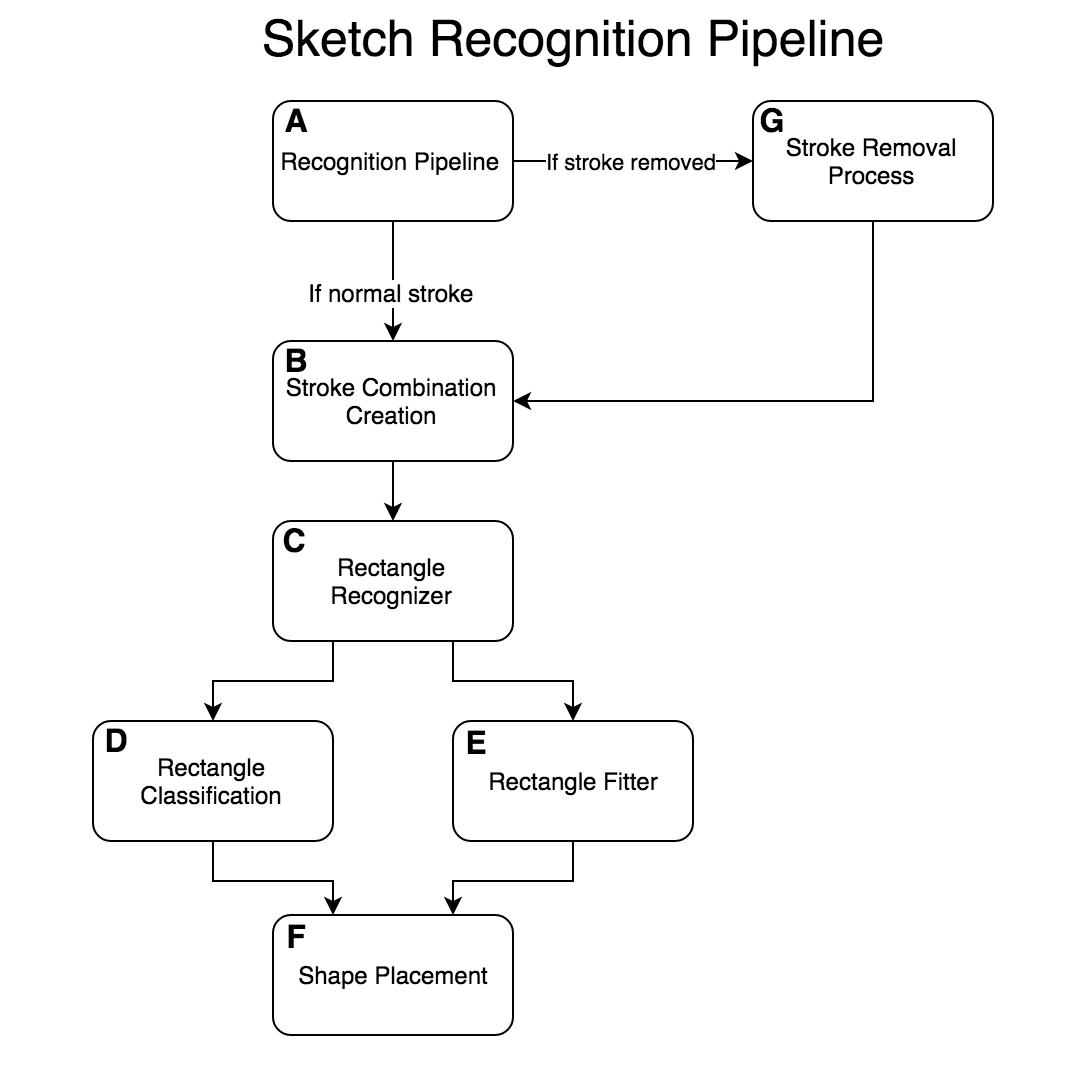
\includegraphics[width=.9\textwidth]{sketchpipeline}
\caption[Recognition pipeline diagram]{Simplified diagram outlining the steps to recognize rectangles from a set of strokes.}
\label{fig:sketchpipeline}
\end{figure}

Once the system has obtained a list of the combinations of strokes that have been accepted as rectangles, it selects the series of objects yielding the highest score to be drawn onto the interface. Afterwards, the chosen sets of strokes are assessed using two algorithms: one for fitting the best possible rectangle, and one for an initial classification type. We attempt to fit rectangles to the user's drawn strokes in order to display our interpretation of the design. The fitting uses a 2D heuristic created from the sum of the overall distance from the proposed rectangle to each one of the points from the user created strokes. Next, a classification algorithm from the system presents the user with an initial type for the newly created object. Finally, the shape is placed on the screen for the user to evaluate and edit. After the conclusion of this pipeline, the user may continue to engage with the interface, repeating the pipeline for each stroke added. Or, the user may conclude editing, which continues onto the rest of the OASIS processes.

%the thought process behind the steps?
%combinations of 4
%why only 4
%how do we pick them
%math of scoring
%angle and distance

\section{Combinations of Strokes}
\label{sec:combostrokes}

While it is possible to generate the score of all subsets given all user strokes, scoring $2^n$ combinations of strokes is inefficient. Also, choosing random sets of strokes does not ensure a sufficient level of accuracy. I propose a scoring algorithm to select particular groupings that maximize the probability of the strokes forming a coherent rectangle. \\

To begin, each stroke is compared with every other stroke. As shown in Equation \ref{equ:comboscoring}, the score between two strokes is determined by their interior angle between the two lines and their distance apart. Each score is recorded and new scores are calculated only when a new stroke is produced by the user or an existing stroke is edited. \\

As shown in Equation \ref{equ:perpendicular}, the \textit{perpendicular} equation penalizes strokes that are not perpendicular with one another. The angles are calculated using the the line of best fit algorithm described in the section \ref{sec:bestfit}. An angle that is a multiple of 45 (but not 90) produces the highest score. A low score indicates a better fit (more similar) to the original stroke.

\begin{equation}
\label{equ:perpendicular}
perpendicular(x,y) = \dfrac{45 - |((x_{angle} - y_{angle})\%90) - 45|}{45}
\end{equation}

The \textit{distance} equation, as shown in Equation \ref{equ:dist}, rewards pairs of strokes with small amounts of distance between them. Distance between two strokes is measured by the smallest Euclidean distance between all combinations of the strokes' endpoints. Nearby and perpendicular strokes represent the types most likely to form a rectangle with one another.

\begin{equation}
\label{equ:dist}
distance(x,y) = \dfrac{endPointDistance(x,y)}{max(canvas_{w}, canvas_{h})}
\end{equation}

The two metrics are summed to create a score representing the probability that two strokes are likely to form a rectangle with one another. A low score represents a high probability of rectangle cohesion, while a high score implies a low probability. Using each stroke's list of scores against all other strokes, we pick from the top scoring strokes to create sets of four for the next process in the recognizer.

\begin{equation}
\label{equ:comboscoring}
Score(x,y) = perpendicular(x,y) + distance(x,y)
\end{equation}

% For each stroke that is added by the user, it is scored against all other strokes. Each stroke records its score against all other strokes in a priority queue. The stroke will later use the top scoring neighboring strokes to create groupings, avoiding other strokes it was unlikely to create an object with.  Ideally, the first 3 strokes will be popped from the queue, and combine with the base stroke to create an object. \\

%SIMILARLITY CHECK
% The before mentioned metrics would allow strokes that are virtually identical score extremely well. However, a rectangle representing a furniture item will rarely contain 2 strokes that are visually the same in both angle and position. Therefore, pairs of strokes scoring below .05 will not be considered. \\

I acknowledge that not all rectangles created by users are created with 4 strokes. However, the metrics needed to define a rectangle drawn with 1, 2, or $n$ strokes adds a new level of complexity to the problem. With any numbers other than 4, the strokes would need to be normalized to 4 with some method. For numbers less than 4, I propose breaking strokes at their corners. For numbers greater than 4, a method to combine similar lines would be needed.

\section{Rectangle Recognizer}
\label{sec:rectrecognizer}

%aka how do we know four strokes are a rectangle, etc.
To recognize a set of strokes as a rectangle, the recognizer works in three basic steps: rejecting groupings that do not pass the threshold for the rectangle metrics, scoring the groups of strokes that do exceed the threshold, and selecting the top scoring groupings as an object. The rectangle metrics are three heuristics that, when passed in conjunction, almost always produce a recognizable rectangle. Even if a stroke belongs to more than one possible set, it may only form an object with the highest scoring set of strokes where all other members do not belong to any higher scoring group. Given a large set of possible combinations, the recognizer selects the best to be created into rectangles.
%choosing of the 4 strokes

%the three checks
\subsection{Rectangle Metrics}
%all are close to lines
%reference the line algorithm from before

This subsection lists and describes the metrics used to identify if a set of strokes is mathematically similar to a rectangle.

\subsubsection{Line Ending Comparison}

The first rectangle metric specifies that all stroke endpoints in the set must be near another unique endpoint within the same set. This metric ensures that the strokes are spatially adjacent and create a closed polygon.

%line ending pairings
\begin{algorithm}
\caption[Function for Line Ending Pairings]{Function detailing the pairings of line endings}
\label{alg:lineendings}
\begin{algorithmic}[1]
\Function{LineEndings}{endPoints, maxDist}
\State $pairs \gets $ []
\For{$i = 0 \to $\textbf{sizeof}$ endPoints - 1 $ }
    \For{$j = i+1  \to$ \textbf{sizeof}($ endPoints $) }
        \State $d \gets distance(endPoints_i, endPoints_j)$
        \If{$d < maxDist$}
            \State $pairs \gets [endPoints_i, endPoints_j]$
            \State \textbf{remove} $i, j$
            \State \textbf{break}
        \EndIf
    \EndFor
    \If{\textbf{sizeof}($pairs$) $<$ \textbf{sizeof}($endPoints$)/2}
        \State \textbf{return} []
    \Else
        \State \textbf{return} pairs
    \EndIf
\EndFor
\EndFunction
\end{algorithmic}
\end{algorithm}

Algorithm \ref{alg:lineendings} outlines the greedy method used to pair the line endings. Endpoints are compared by distance and paired with the first choice within the maximum distance allowed.

\begin{equation}
\label{equ:maxdistcorners}
maxDist = \dfrac{p}{n} \cdot \sum_{i=0}^{n-1} length(stroke_i)
\end{equation}

Equation \ref{equ:maxdistcorners} describes a formula to determine the maximum distance allowed between endpoint pairings given $n$ strokes and percentage of stroke length $p$. I used a percentage of .1, the desired maximum distance between endpoints was 10 percent of the average length of strokes involved. 

\subsubsection{Line Straightness}
The second rectangle metric states that all strokes in a rectangle object must be similar in straightness to a line. To determine this, I use the LengthRatio described in Equation \ref{equ:ratio3}. The purpose of this metric is to ensure there exists no odd edges or irregularities; a wavy line will receive a poor score when comparing similarity against the straight edge of a rectangle. While I did use .95 as a threshold for a line when sketching walls, I used a .9 threshold for this metric to allow for a little more flexibility.

\subsubsection{Perpendicular Angles}

A property of all rectangles is that all interior angles equal 90 degrees. Therefore, the last rectangle metric is the average interior angle of the set of strokes.\\

\begin{equation}
\label{equ:angle2strokes}
\theta = tan(\dfrac{|slope_i - slope_{j}|}{1 + (slope_i \cdot slope_{j})})
\end{equation}

\begin{equation}
\label{equ:center}
\begin{aligned}
center_x = \dfrac{1}{n} \cdot \sum_{i=0}^{n} stroke_i.x
\\[1pt]
center_y = \dfrac{1}{n} \cdot \sum_{i=0}^{n} stroke_i.y
\end{aligned}
\end{equation}

\begin{equation}
\label{equ:anglecenter}
\theta = tan(\dfrac{stroke_y - center_y}{stroke_x - center_x})
\end{equation}

Shown in Equation \ref{equ:angle2strokes} is the formula used to calculate the interior angle given two strokes, $i,j$. The slopes of the strokes are calculated using the line of best fit algorithm described in the previous chapter. 

%right angle check
\begin{algorithm}
\caption[Function to check for right angle between strokes]{Function to check for right angles between strokes}
\label{alg:rightangle}
\begin{algorithmic}[1]
\Function{rightAngles}{strokes, threshold}
\State $angles \gets $ []
\State $n \gets $\textbf{sizeof} ($strokes$)
\State $s \gets $ \textbf{sort}(strokes, angleAwayFromCenter)

\For{$i = 0 \to $\textbf{sizeof} ($strokes - 1$)  }
    \State $angles \gets  angle2Lines(strokes_i, strokes_{(i+1)\%n})$
\EndFor
\State $sum \gets $(\textbf{sum}(angles)) / n
\If{$\left|sum - 90\right| <$ \textbf{sizeof}($endPoints$)/2}
        \State \textbf{return} true
    \EndIf
\State \textbf{return} false

\EndFunction
\end{algorithmic}
\end{algorithm}

The function to calculate this average is described in Algorithm \ref{alg:rightangle}. One important step noted in the algorithm is the ordering of the strokes by their angles with respect to the center of the set of strokes. The formula used to calculate the angle from the center is shown in Equation \ref{equ:anglecenter}. Given the strokes are in order, the strokes will be compared adjacently, resulting in the calculation of the correct interior angles.

\subsubsection{Alternate Solution}

An alternative method of recognition that was implemented but not used was a design based heavily on using the \$N recognizer by Anthony and Wobbrock \cite{dollarN}. Using the same combination creation algorithm, the strokes would be processed by the \$N recognizer instead of my recognizer. The strokes would be compared to a template dataset of rectangles and letters. However, since the \$N recognizer accounted for direction of drawn strokes as well as the ordering, the number of combinations checked was orders of magnitude higher than my implementation. Due to the sheer number of combinations checked, the \$N recognizer often found combinations of strokes that scored well on different templates than intended. Although it was possible to better choose combinations for the recognizer to analyze, the recognizer was being modified for a purpose it was not designed to handle, and that the recognizer was not being used for its strengths anymore. The \$N recognizer's strengths were its flexibility in recognizing any number of symbols in its data set, and ease of incorporation into any Javascript-based program. With the small amount of objects in the data set, its flexibility was no long valued. Since the shapes recognized in this system can be of any size and rotation, the \$N also has a difficult time matching them to its fixed sized and proportioned templates. In addition, all the modifications the recognizer needed to rework it for our purposes removed any ease of importing it once had.

\section{Classification}
\label{sec:classification}

%use the ratio from the templates
%find the closest one

The classification of an object entails assigning it a set of attributes to define itself, such as a name, type, and color. I classify objects based on their ratio compared to the ratios created by dimensions of real world objects. \\

In Table \ref{table:furniture}, I list the actual height and width of furniture items, as well as their pixel equivalents. I chose 200 pixels to represent 80 inches, however the number is fairly irrelevant since the primary comparisons are between ratios, which are unit independent. Skylights are not included due to their arbitrary size and shape. Users must manually classify a skylight in order to create one. \\

When a user creates a series of strokes and it is properly identified as a rectangle by the recognizer, it is sent to the rectangle classifier to receive a classification. The user's height to width ratio of his/her drawn furniture items compared to those of real objects \cite{dimensions}. The ratio of height to width (in pixel values) of the the rectangle is compared to each of the ratios of the furniture items. The closest percentage is chosen as the classification shown to the user. As stated in the previous chapter, users may reclassify any furniture item by either right clicking and selecting a menu item, or sketching the appropriate letter on top of the object. \\

\begin{table}[]
\centering
\caption{Furniture height to width comparisons}
\label{table:furniture}
\begin{tabular}{|l|l|l|l|l|l|}
\hline
 & Pixel Height & Pixel Width & {Height (in)} & {Width (in)} & Ratio ($\dfrac{h}{w}$) \\ \hline
Bed (twin) & 97.5 & 187.5 & 39 & 75 & 0.5200 \\ \hline
Bed (full) & 135 & 187.5 & 54 & 75 & 0.7200 \\ \hline
Bed (queen) & 150 & 200 & 60 & 80 & 0.7500 \\ \hline
Bed (king) & 190 & 200 & 76 & 80 & 0.9500 \\ \hline
Desk & 75 & 150 & 30 & 60 & 0.5000 \\ \hline
Wardrobe & 150 & 200 & 60 & 74 & 0.8108 \\ \hline
\end{tabular}
\end{table}

\section{Rectangle Fitting}
\label{sec:rectfitting}
%jiggling that slows down a bit

Finally, after the rectangle is recognized and chosen, a rectangle is fitted to the set of strokes. First, a small rectangle is placed at the center of the strokes as the first iteration of the rectangle. The growth of the rectangle will iterate though using the following algorithm:

% \begin{algorithm}
% \caption{Rect-Score(points, rectangle)}
% \begin{algorithmic}[1]
% \State $s \gets 0$
% \State $ro \gets$ Rotate-Points $(points, center, angle)$
% \For{$rpoint$ \textbf{in} $ro$}
%     \State $s \gets s + rectDistance(center, rect, rpoint)$ \Comment{rpoint = rotated point}
% \EndFor
% \State \textbf{return} $o$
% \end{algorithmic}
% \end{algorithm}

\begin{algorithm}
\caption{Rectangle-Scoring(points, rectangle, pScore, Inc)}
\begin{algorithmic}[1]
\State $s \gets $[ ]
\State $r \gets  $Wiggle$(rectangle, inc)$
\For{\textbf{each} $rect$ \textbf{in} $r$}
    \For{\textbf{each} p \textbf{in} $points$}
        \State $s \gets s$ + Rect-Distance(center($points$), $rect, p$)
    \EndFor
\EndFor
\State $s \gets sort(s)$ \Comment{Sort by pScore, lowest to highest}
\If{s[0].pScore $<$ pScore}
    \State \textbf{return} Rectangle-Scoring($points, s[0], s[0].pScore, Inc + 1$)
\Else
    \State \textbf{return} $s[0]$
\EndIf
\end{algorithmic}
\end{algorithm}

First, the rectangle is 'wiggled' using the Wiggle function. This creates up to 10 rectangles based on changed attributes. Using those proposed rectangles, the function scores each one of them using the Rect-Distance function outlined in Algorithm \ref{alg:rectdistance}. Next, the rectangle with the lowest score is chosen and compared with the current score. If the score is lower, then a next iteration is performed. If the score is higher, then the function ends and the current rectangle is chosen.

% \begin{enumerate}
%     \item 'Wiggle' the rectangle in all possible directions and rotations.
%     \item Score each rectangle created by the different attribute changes.
%     \item Of all movements, take the best score.
%     \item Compare the new score with the score of the initial rectangle from the beginning of this iteration.
%     \begin{enumerate}
%         \item If the score is lower (better), the cycle repeats, starting from Step 1 with the new rectangle as the current iteration.
%         \item Otherwise, the function stops.
%     \end{enumerate}
% \end{enumerate}

Algorithm \ref{alg:wiggle} describes how the W¬iggle function changes the rectangle. Each property of the rectangle is increased or decreased: height, width, x position, y position, and angle. From each attribute changed, a new rectangle is created. Only one attribute is changed per iteration to accurately determine each characteristic's effect on the score. The system starts with a coefficient that determines the increments per iteration. In the beginning, the coefficient is high, resulting in a high increment. Early iterations of the rectangle are unlikely to score well, so less precision is necessary in initial steps. As the number of iterations increases, the coefficient decreases as the rectangle approaches the optimal size. The increments between angle and length/width/position are the same. When the increments become their smallest smallest, all increments are of size one.\\

\begin{algorithm}
\caption{Wiggle(rectangle, count)}
\label{alg:wiggle}
\begin{algorithmic}[1]
\State $o \gets$ [ ]
\State $i \gets $\textbf{roundUp}(StartInc/count)\Comment{StartInc = 50}
\For{variable in rectangle}
    \State $a \gets rectangle_{variable}+i$
    \State $b \gets rectangle_{variable}-i$
    \State $o \gets a,b$
\EndFor
\State \textbf{return} $o$
\end{algorithmic}
\end{algorithm}

% Each rectangle produced by the Wiggle function is scored against the points in the chosen set of strokes. To score a rectangle against all the strokes, the system sums the individual scores from each point. The algorithm used to calculate a score for individual point is shown in Algorithm \ref{alg:rectdistance}.

%overall score of a rectangle
% \begin{algorithm}
% \caption{Rect-Score(points, rectangle)}
% \label{alg:rectscore}
% \begin{algorithmic}[1]
% \State $s \gets 0$
% \State $ro \gets$ Rotate-Points $(points, center, angle)$

% I calculate the distance between each point among all strokes in the set to its closest point on the iteratively growing rectangle. \\

% \For{$rpoint$ \textbf{in} $ro$}
%     \State $s \gets s + rectDistance(center, rect, rpoint)$ \Comment{rpoint = rotated point}
% \EndFor
% \State \textbf{return} $o$
% \end{algorithmic}
% \end{algorithm}

The distance is calculated between each point contained within the lines and the rectangle is outlined in Algorithm \ref{alg:rectdistance}. The points compared are the points obtained from resampling described in section \ref{sec:resample}. A lower score indicates a better match, since the score is the sum of distance away from the rectangle. There are 3 cases where the point exists in relation to the rectangle: outside the rectangle, inside the rectangle, or perfectly on the line. Given the point is outside the rectangle, the score is the distance from the edge of the rectangle to the point. If the point is on the rectangle's edge, the score is 0. If the rectangle is on the inside of the rectangle, the system uses the distance to the closest edge of the rectangle. \\

%the distance from one point to the rectangle
\begin{algorithm}
\caption{Rect-Distance(centroid, rectangle, point)}
\label{alg:rectdistance}
\begin{algorithmic}[1]
\State $dx \gets max(|point_x - centroid_x|-(rectangle_w/2), 0)$
\State $dy \gets max(|point_y - centroid_y|-(rectangle_h/2), 0)$
\If{dx=0,dy=0}
    \State \textbf{return}
    $min(|point_x - centroid_x|-(rectangle_w/2),
    |point_x - centroid_x|+(rectangle_w/2),
    |point_y - centroid_y|-(rectangle_h/2),
    |point_y - centroid_y|+(rectangle_h/2))$
\Else
    \State \textbf{return} $\sqrt{dx^2 + dy^2}$
\EndIf
\end{algorithmic}
\end{algorithm}

Since it is comparatively difficult to calculate the distance between a point and a rotated rectangle, the points are rotated instead. The rectangle is kept orthogonal, but other attributes are applied normally. All points are rotated with respect to the center of the set of strokes. The method to rotate all points is given in Algorithm \ref{alg:rotatepts}. \\

%rotates the points
\begin{algorithm}
\caption{Rotate-Points(points, rectangle)}
\label{alg:rotatepts}
\begin{algorithmic}[1]
\State $q \gets []$
\For{$p$ \textbf{in} $points$}
    \State $ca \gets cos(rectangle_a), sa \gets sin(rectangle_a)$
    \State $dx \gets p_x-rectangle_{cx}, dy \gets p_y-rectangle_{cy}$
    \State $p_x \gets ca*dx-sa*dx + rectangle_{cx}$
    \State $p_y \gets sa*dx+ca*dy + rectangle_{cy} $
    \State $q \gets p$
\EndFor
\State \textbf{return} $q$
\end{algorithmic}
\end{algorithm}

\begin{figure}[ht]
\centering
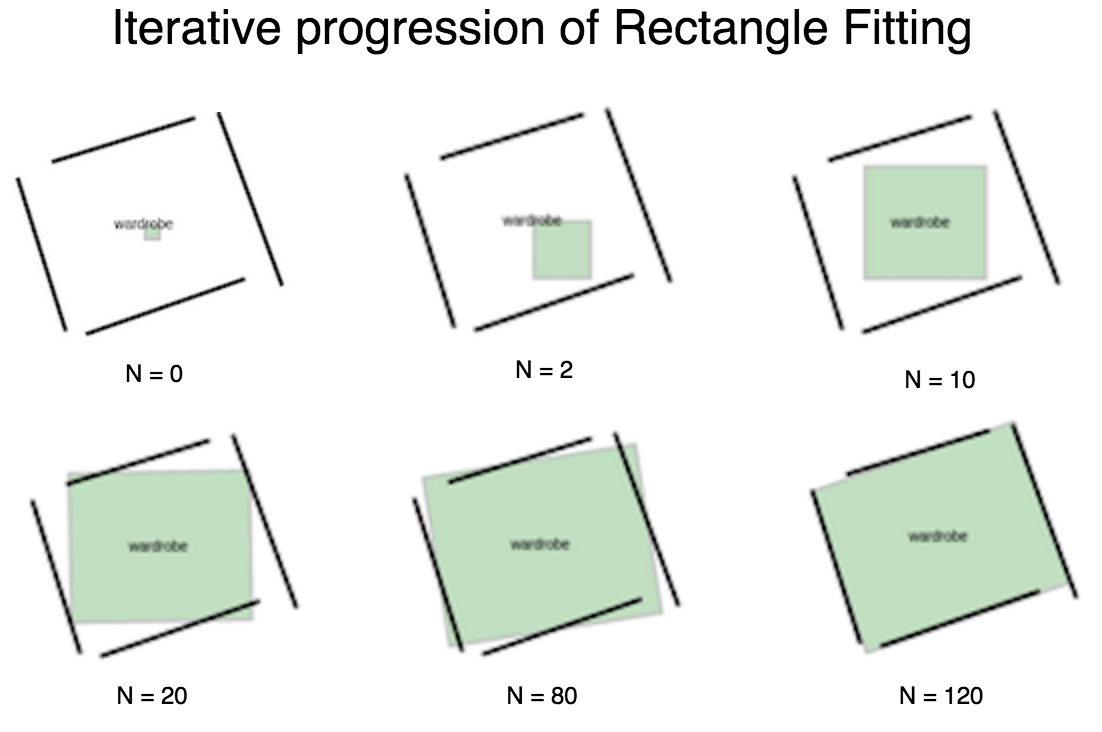
\includegraphics[width=\textwidth]{fitting}
\caption[Iterative step images taken during the rectangle fitting process]{Images taken a different timestamps in the process of iterative fitting.}
\label{fig:fitting}
\end{figure}

After each rectangle created by Algorithm \ref{alg:wiggle} is scored using the before mentioned algorithms, the best scoring iteration is compared to the current iteration. If the new iteration scored better, it becomes the new iteration, and the process repeats. If the current iteration is better, the system has determined that it cannot edit the rectangle any further to create a better scoring result. Therefore, it stops iterating and proceeds to produce a rectangle on the canvas for the user to see. \\

After the rectangle stops iterating, the object has settled in a local minima for score. There is a possibility that it is not the global minima, and that it has settled for a lesser scoring rectangle. Nonetheless, it is acceptable for the rectangle to settle in a local minima since the accuracy is not application breaking. 

\section{Stroke Removal}
\label{sec:strokeremoval}

The removal of strokes presents an interesting problem in this system. As stated in the previous chapter, removal of elements may be done in one of two ways: scribbling and overdrawing. When a stroke is removed by the user, the classifications involving that stroke are no longer valid, as shown in Figure \ref{fig:deleteclass}.

\begin{figure}[ht]
\centering
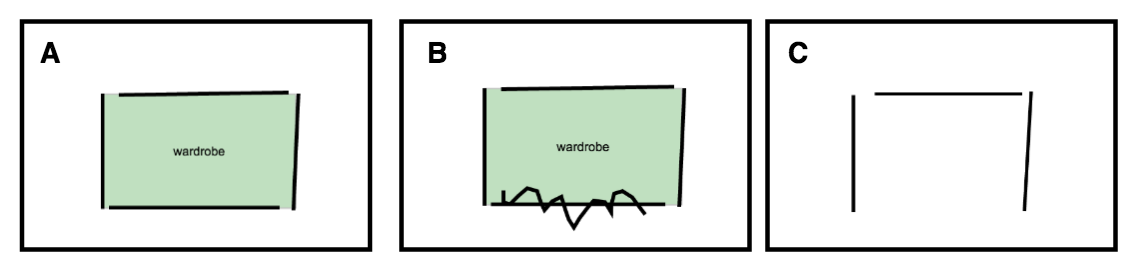
\includegraphics[width=\textwidth]{deleteclass}
\caption[Removal of objects when a stroke is removed]{A diagram depicting the the removal of the object when one of its strokes has been deleted.}
\label{fig:deleteclass}
\end{figure}

As shown in Figure \ref{fig:sketchpipeline}-G, deleting a stroke alters the pipeline slightly. First, the stroke itself must be removed from the interface. Next, all classifications and recognized shapes associated with the removed stroke must also be discarded. If the stroke was not associated with any recognitions, there is no further need to reprocess. However, the removal of those classifications implies that the strokes who used to belong to that recognized object are available. Therefore, we must reprocess the sketch to search for other possible shape recognitions that may be possible.

To start reprocessing the image, stroke combinations are created once again minus the stroke that was removed. The system attempts to readd all strokes that were effected by the removal of one of the strokes. This allows the system to attempt to find new recognized rectangles, if the removed stroke had not existed. Afterwards, the process remains the same as if the process had begun with a new stroke, except using different combinations.

\section{Reclassification}
Furniture items are created via recognition of a viable rectangle present. whose method of creation I will discuss in further detail in the next chapter. However, what will be presented now is the usage of furniture items during sketching, and its available actions and properties.

\begin{figure}[ht]
\centering
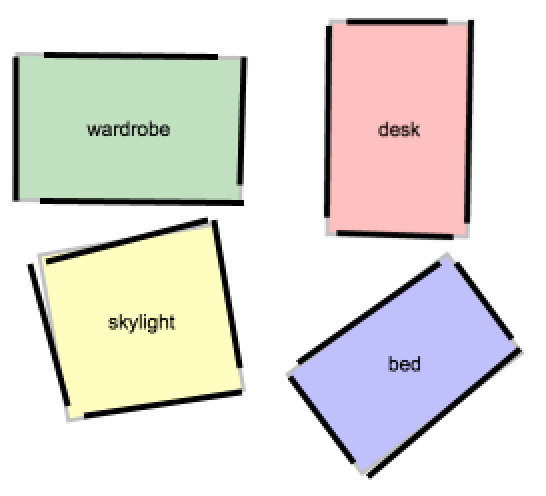
\includegraphics[width=.5\textwidth]{furniture}
\caption[Examples of recognized objects]{Examples of recognized objects. Each piece of furniture or skylight is colored differently, as well as labeled.}
\label{fig:furniture}
\end{figure}

After being recognized, a rectangle is fitted to the strokes. That rectangle may be moved by double clicking and dragging it, also translating its base strokes along to its new location. Objects may not be moved outside the sketching interface boundaries. \\

The rectangle will be assigned an initial classification. Classifications include types of furniture, such as a bed or wardrobe. If the user disagrees with the system's initial classification, the user has two methods of overriding it. First, the user may right-click any object, as shown in Figure \ref{fig:reclassify}, and a menu will appear. The user can reclassify the object as a different object by selecting any of menu items. The only attributes that are modified are the name, type, and color of the object.

\begin{figure}[ht]
\centering
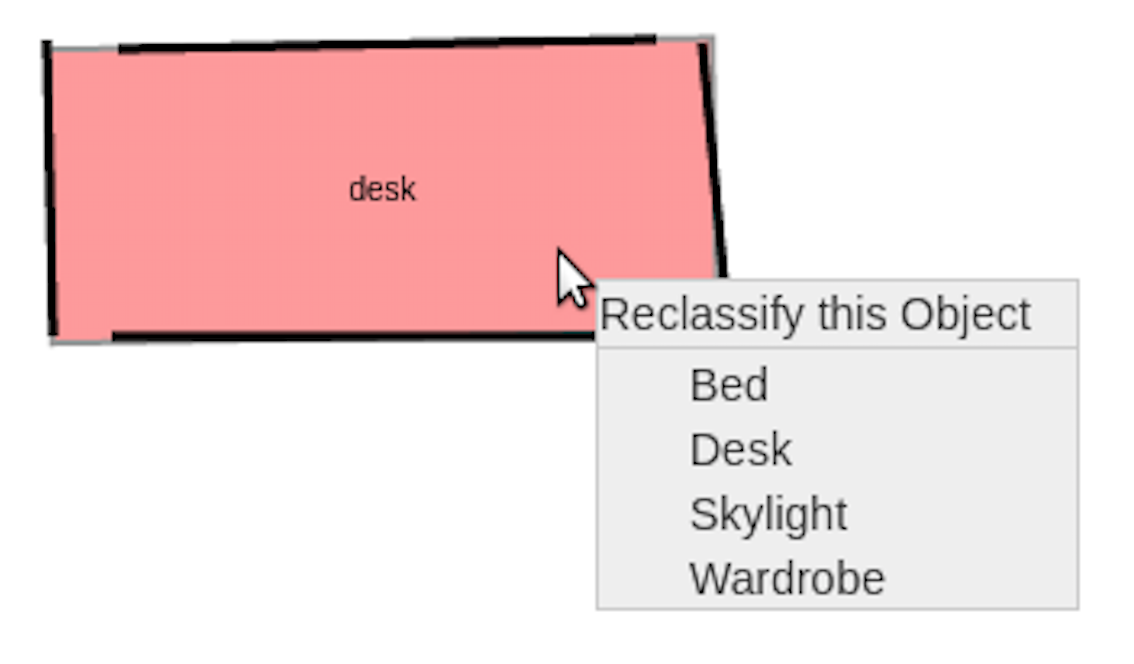
\includegraphics[width=.5\textwidth]{reclassify}
\caption[Image of the reclassification menu]{Upon right clicking on an object, a menu is shown to the user.}
\label{fig:reclassify}
\end{figure}

A second method the user has to reclassify an object is to sketch the corresponding letter on top of the object. The corresponding letter is the first letter of the desired classification, such as the letter 'W' if the user would like to reclassify an object to a wardrobe.

\begin{figure}[ht]
\centering
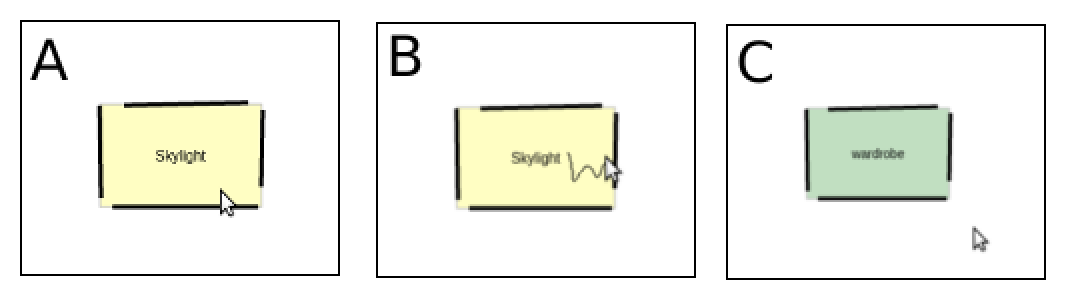
\includegraphics[width=\textwidth]{reclassifydraw}
\caption[Example of reclassification with recognition]{Upon drawing the correct corresponding letter, the user can reclassify an object to another classification.}
\label{fig:reclassifydraw}
\end{figure}

This recognition works by using the \$N recognizer, as described in chapter 2. Using a set of templates corresponding to the first first letters of each of the types of objects, the newly added stroke is processed by the recognizer to check if it matches with any letters. If it is a confident enough match, and the stroke is within the boundaries of an object, then that object is now reclassified to the new type of object. Afterwards, the classification stroke drawn to classify the object is removed and no longer shown. \\

Each method of reclassification has its merits. The right-click menu is more accurate and less reliant on interpretation, since there is no guesswork needed. The letter recognition is arguably faster and intuitive, but has a much larger margin for error. There exists the possibility of the letter not being recognized, or even recognized as the incorrect letter. With the availability of two methods, the user has even more flexibility and choice with his/her designs. 
%reprocessing the image as if that stroke had not been drawn. 

\section{Chapter Summary}
In this chapter, we reviewed how the system selects combinations of strokes to use in the recognizer, and used scoring functions used to determine the existence of a user drawn rectangle. Afterwards, a method of classification based only on stroke dimensions was presented. Finally, I outlined the procedure used to accurately fit a rectangle to a set of user drawn lines. The following chapter discusses the outline and analysis of a brief pilot study based on this system.
    %%%%%%%%%%%%%%%%%%%%%%%%%%%%%%%%%%%%%%%%%%%%%%%%%%%%%%%%%%%%%%%%%%%
%                                                                 %
%                            CHAPTER FIVE                          %
%                                                                 %
%%%%%%%%%%%%%%%%%%%%%%%%%%%%%%%%%%%%%%%%%%%%%%%%%%%%%%%%%%%%%%%%%%%
\chapter{Pilot User Study} \label{sec:pilot}

In the previous chapters, I described in detail the modifications to OASIS and the rationale behind those changes. In order to confirm the validity of this work, I performed a small pilot user study on 6 students aimed at determining the usability and accuracy of this sketching interface compared to the classic interface on OASIS. This chapter will outline and briefly analyze the feedback received from those participating in the study.

\section{Study Conditions and Methods}
%how were they asked (phone, in person)
%under what conditions did they perform the study
%how much did I guide them

%guidelines I tried to follow

Participants participated in one of two scenarios: in person questioning or over the phone. I attempted to keep the experience the same for both types of participants. Those that partook in person had access to a Wacom Intuos CTL490DW digital drawing tablet, and those who participated over the phone did not. Aside from a brief overview of the project itself, all users were guided minimally once logged onto OASIS. However, I was available for guidance throughout the study and answered all questions to the best of my ability. All participants were asked to draw a room of their choice on each of the user interfaces. The first interface, the drag-and-drop interface is the `classic` version of the interface. The second interface is the sketching interface, and emulates sketching with a pencil. Participants were allowed design on the interfaces in any order. Neither interface design proceeded past the design phase, and did not proceed to the 3D model generation. Afterwards, all participants were asked the same series of questions about their experience. 

\section{Questions and Goals}
The following questions were asked to each of 6 participants after each design, and their responses were recorded. The primary goals of this user study are to isolate the positives and negatives from both systems, learn from them, and apply them accordingly to improve OASIS. Since most of the development of this thesis has been done in isolation, it is enlightening to gather feedback on my work. Another goal is to learn more about other users' perceptions of the interface's usability, and if anything is unclear or confusing. Finally, one last goal is find areas of improvement and new features that users desire in such a system.

\subsection{Questions}
\begin{enumerate}
\item Questions per user:
\begin{itemize}
    \item If any, do you have any experience or formal education in architecture or visual arts? If so, which one and how many years?
    \item Do you have experience with modeling software? If so, which ones?
\end{itemize}
\item Questions per user interface, per design:
\begin{itemize}
    \item On a scale of 1 to 5 (5 being the most confident), how confident are you in your accuracy of design? (dimensions, scale, layout) Why is this your score?
    \item If anything, what did you find fun or interesting about this sketching environment?
    \item Describe designs you were unable to create due to system limitations.
    \item Was there anything you did not like about working in this sketching environment?
    \item Were there any parts of the interface that were hard to use or confusing?
\end{itemize}
\item Questions only for the new sketching interface:
\begin{itemize}
    \item Describe your impressions of the system’s effectiveness in interpreting your design.
    \item Rate on scale of 1 to 5 (5 being the highest), the accuracy to which the system displayed your design, based on your intentions. Why is this your score?
\end{itemize}
\end{enumerate}

\section{Responses and Analysis}
The before mentioned process was conducted with group of fellow students of mixed backgrounds. No students that participated had any familiarity with either system, or any formal experience with architecture. Overall, feedback on the sketching interface was mixed. Users appreciated the flexibility and freedom the new interface offered, but still felt it was lacking in possible features. There was a general concensus that a lack of directions or list of available actions made it difficult to use at first. However, most users agreed it was relatively enjoyable to use and showed potential. Below are some direct quotes about the new system offered by the participants:

\begin{itemize}
    \item Positives:
    \begin{itemize}
        \item  "I thought it was pretty cool, I could draw whatever shapes I wanted".
        \item "It's pretty awesome to scribble stuff out."
        \item "After using the new system, I felt more constrained [in the old system] in terms of what I could make. I couldn’t make the furniture whatever size I wanted."
        \item "Overall it’s pretty fun [...] I thought it would be like Microsoft paint but its like a step beyond that."
        \item "It's pretty fun to just draw stuff and scribble it out."
    \end{itemize}
    \item Negatives:
    \begin{itemize}
        \item "The shapes it can recognize are too limited, what about other shapes like circles and triangles?"
        
        \item "Sometimes it wouldn’t recognize a rectangle that I’m pretty sure is a rectangle."
        
        \item "The classifications on furniture and stuff seemed pretty random."
        
        \item "It feels flexible but limited at the same time, I felt like I could draw anything but the system couldn't handle everything."
        
        \item "I was confused at first what it could do and what I could do."
        
    \end{itemize}
\end{itemize}

\begin{figure}[ht]
\centering
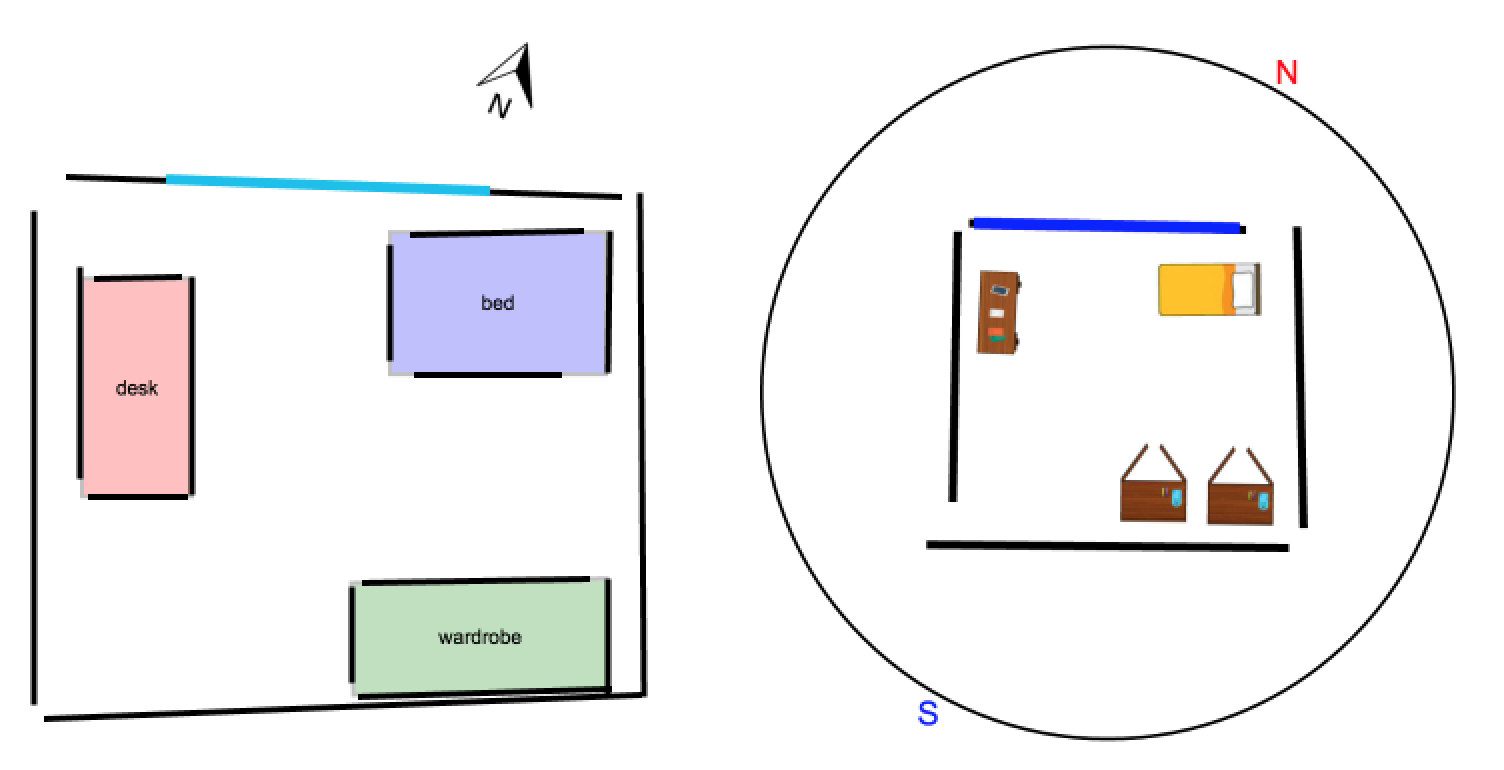
\includegraphics[width=\textwidth]{comparison}
\caption[Comparison of user designed models]{Shown above are two models created by the same user of the same room.}
\label{fig:comparison}
\end{figure}

An overwhelming concern with the new system was its lack of in-system guidance and assistance. Where the classic system had a help menu and instructional video, no similar support was available for the new sketching interface. This caused initial confusion and indecisiveness amongst all participants. However, as the users discovered and learned about its features, most embraced the possibilities it offered.

\begin{figure}[ht]
\centering
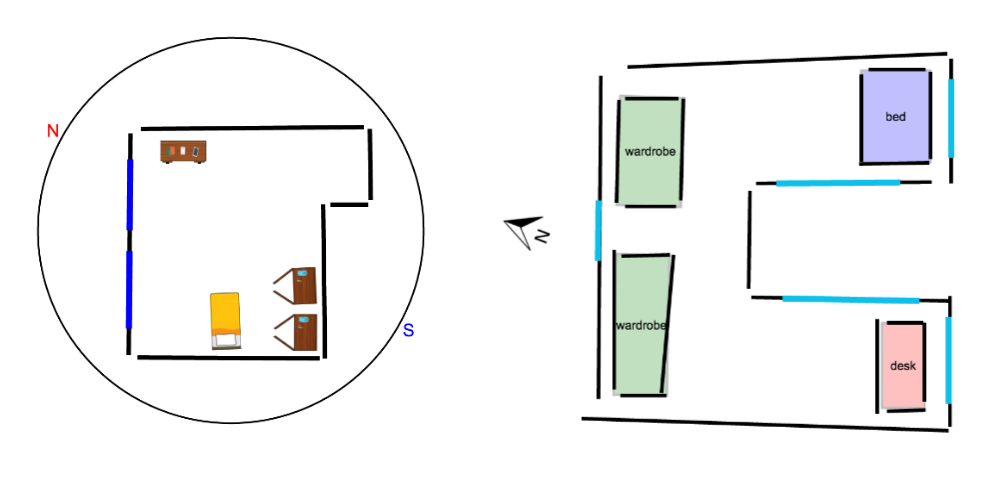
\includegraphics[width=.9\textwidth]{userdrawings}
\caption[Additional user created drawings for the pilot study]{Shown above are two additional models created by users who participated in the study.}
\label{fig:moredrawings}
\end{figure}

Visually, comments were made concerning the lack of images in the new interface. The classic interface overlaid an image of the furniture, clearly indicating what type of furniture it was. The sketching interface had a labels and colors, but the participants found it more visually pleasing to look at images instead of monochromatic blocks. \\

\begin{figure}[ht]
\centering
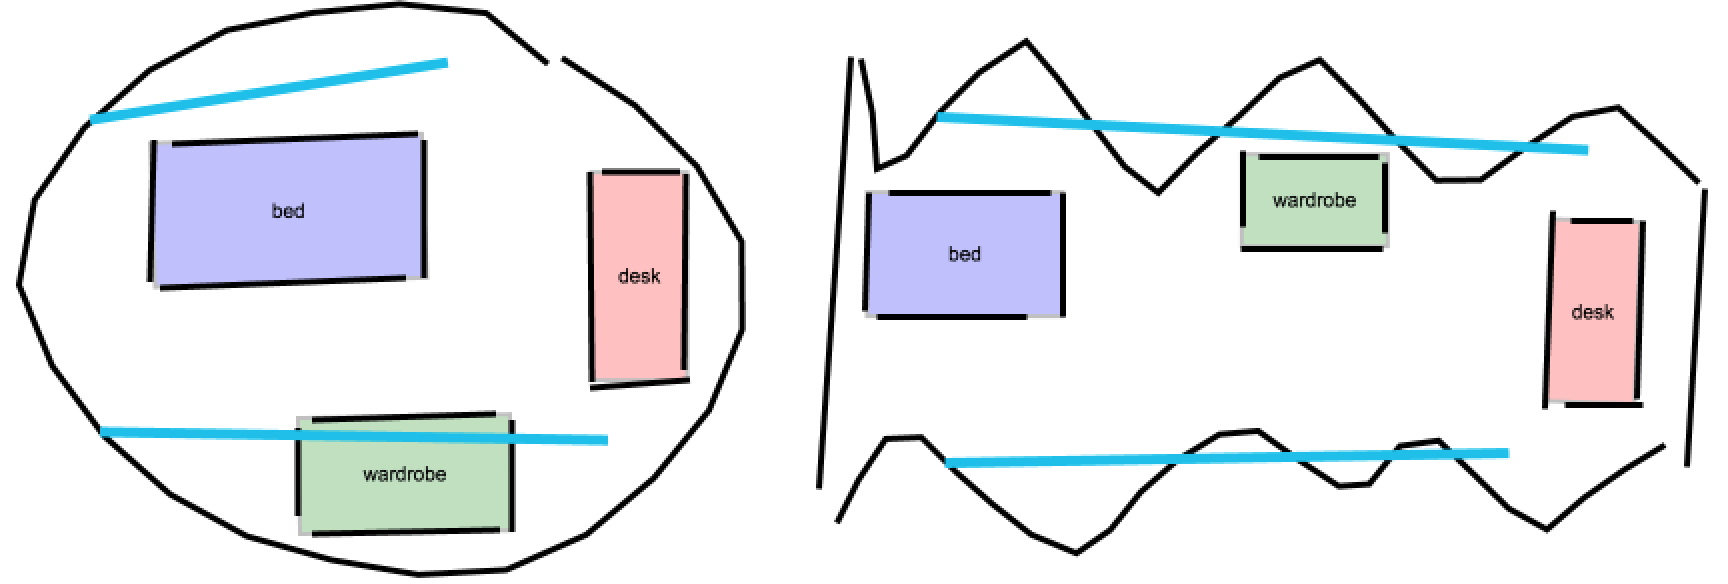
\includegraphics[width=.9\textwidth]{badwindows}
\caption[Examples of windows not snapping correctly]{Shown above are two models where the windows did not snap correctly to the walls they were attached to.}
\label{fig:badwindows}
\end{figure}

The order in which the participants chose to use the interface seemed to have a surprising impact on their feedback. Those that chose the new sketching interface first felt more constrained in their available design choices once they started using the classic interface. The users that chose to use the classic interface first seemed more conservative in their design choices. Typically, the interface that was chosen second received more criticism. Since no users had any prior experience with systems such as this, it made logical sense that the first interface they used became the baseline for their sense of comparison.

There were some types of models I was not prepared for, and most problems stemmed from the lack of flexible windows. Two examples are shown in Figure \ref{fig:badwindows}, the left is a single, curved stoke as the surrounding wall, while the right drew a jagged edge as a whole wall. As explained in chapter 3, the window snapping algorithm uses the line of best fit of the wall it is attempting to attach to. This approach works well for straight lines. However, for strokes similar to an ellipse and highly jagged lines, the result is clearly faulty. I was the primary user of this system during development, and it never occurred to me to even attempt to create a wall for a building that was not straight, let alone attach a window to it. This result only reiterates the importance of user studies. We as developers cannot anticipate the actions of the user, and through studies such as this we can make our systems more robust.

Overall, this pilot study gave a sense of other users' opinions of the system, as well as some welcomed initial feedback. However, in the event of a more detailed user study, there must be a greater attention to detail. If a proper user study is to be conducted, more details about each participant must be recorded. A greater variety of participants is also necessary to gain a broader variety of opinions. Recording details about the usage of the system and each user's actions would allow a more in-depth analysis of the system. This pilot study made some good first steps, but further adjustments must be made for a more comprehensive user study.

\section{Chapter Summary}

This chapter summarizes a brief pilot study performed to determine the effectiveness of this work against the previous user interface of OASIS. Results and feedback were diverse, clearly showing where this work has succeeded and failed. Through the lessons learned in this study, I have identified areas of improvement and possible features for the future. 
    \chapter{CONCLUSION AND FUTURE WORK} \label{sec:conclusion}

\section{Conclusion}

My contributions include the creation of a sketch-based interface for architectural design, modifications and enhancements to OASIS, and the conduction of a pilot study and analysis. The development of the sketching interface included creation of a recognizer, metrics to score various aspects of user drawn strokes, and a novel user interface. Also created were two different methods of reclassifying objects and  a process to fit a rectangle to a set of strokes. Improvements to OASIS include bug fixes, small feature development, and improvements to user experience. The pilot study indicates that the interface does lack some features and depth of available primitives for designers to use. However, the new sketching interface does show promise, and is unique in concept and execution.

\section{Future Work}
\subsection{Dynamic Recognition}
%able to recognize new shapes and figure on the fly

A limitation of this system is its lack of flexibility in recognizable primitives. As shown in the pilot study, users showed desire for the system to recognize additional shapes. While the recognition of rectangles was relatively well received, the shortage of alternative choices for design was received as disappointing. Without extensive further development, the procedure to add more primitives would be time intensive. Currently, the system is limited to recognizing one shape (rectangles), and prior experience has shown that over-reliance on the \$N recognizer in an attempt to recognize too many primitives is ineffective in accomplishing our goals. There is future work to be done to expand the number of recognizable primitives and ease the process of adding those primitives.\\

Not only was the absence of additional shapes noted, but the low flexibility in choice of room items was observed by the participants of the study. All furniture items created were the same shape, with limited customizable attributes. While some users were satisfied with the options, more support should be given to increased number of primitive choices. \\

Research into machine learning based methods may prove to be worthwhile. While machine learning requires significantly more time and data to train, the increased accuracy and reliability reflect that time investment. Using training data that includes new primitives may be a relatively simple solution to the otherwise difficult problem of adding new shapes to the system. The amount of knowledge required to adjust a machine learning algorithm effectively is undeniably high, but it could be a worthwhile investment in the long term.

\subsection{Group Sketching}
Architectural designs are often not created by one person alone, but the culmination of multiple designers' efforts combined. The ability to share and collaborate with other people would be an invaluable tool. With multiple collaborators, models could be more complex and intricate. There exists interesting design choices involving the ownership and versions of models. \\

Currently OASIS and this sketching interface only allow for the ownership of a model to belong to one person. It may be beneficial to adopt version control to assist in organizing models. Version control would allow users to work on models at their own pace, and merge models together to create significantly more complex designs. Additionally, outside of the model viewer, there is no ability to share models with other users. OASIS does contain unique link sharing for models, but it is view-only and does not allow editing. A possible solution would be to allow users to manage the accessibility of their models, allowing each individual user to choose to keep models private or allow other certain other users to edit their models. \\

One possible feature for group sketching would be the adoption of real-time collaborative sketching. The current iteration of this sketching interface does not allow for multiple users to sketch on one interface. Multiple users being able to draw on the same canvas in real time would be a novel feature to add to the sketching interface. However, such a system has its own challenges, such as updating multiple canvases across multiple systems and communicating intent across many users.

\subsection{Multiple View Sketching}

The current sketching interface only allows the user to edit their design in one view: top-down. The locked view from top-down restricts the amount of control and freedom designers have over models. As discussed in chapter 1, there exists many more types of architectural sketches. Views such as isometric, cross section, and elevation can empower users to develop their ideas further. Viewing models from different angles allows the user to better understand the look and feel of what they are designing. Should more viewing angles be available, users could tackle a design problem from multiple angles, sparking more ideas and lead to increased creativity in solutions. \\

For example, by extending to a cross section view, the user can modify the heights of objects. By editing an elevation sketch, a user can adjust how the facade of their room looks. Future work is recommended to explore the area of sketching from multiple views and editing more properties of the model.

\subsection{Pilot Study Improvements}

A more thorough and carefully planned user study could be done to study any number of habits related to sketching. One limitation of the pilot study performed was its low number of participants. I performed the study on a small, select group of users, and it is possible the group I chose suffered from bias due to my involvement in the applicant. Opening the study to all willing applicants would reduce the bias in feedback. Due to a low number of participants, there was a small amount of feedback. Collecting more feedback would allow us to more accurately rate our tool. Another modification to the procedure would be to perform the pilot study for longer. The study lasted only one session, consisting of roughly 15 minutes of application usage and questioning per user. This was far shorter than the time spent conducting the OASIS pilot study \cite{oasis2016}. \\

The amount of information gathered from the participants was limited to the questions asked and models drawn. More information could be gathered and analyzed, such as number of incorrect recognitions or number of edits. Further analysis could be done on user behaviors, including what part of a room users typically draw first, or even the extent to which the designs are to scale. The possibilities to discover interesting patterns within design are endless. 

% \subsection{Expansion to other types of simulations}

% Just as professional CAD software is not limited to architecture design, OASIS and the new sketching interface are not limited to simulating daylight. Since the models created are watertight, it is possible to simulate intangibles such as fluids and sounds. All forms of modeling can benefit from a more productive early design phase. However, OASIS is currently not built to handle simulations other than daylight.

% Improvements to the sketching interface 

% This future work would also be a massive undertaking, expanding not only the sketching interface, but the backend of OASIS as well.


    %%%%%%%%%%%%%%%%%%%%%%%%%%%%%%%%%%%%%%%%%%%%%%%%%%%%%%%%%%%%%%%%%%%
%                                                                 %
%                           BIBLIOGRAPHY                          %
%                                                                 %
%%%%%%%%%%%%%%%%%%%%%%%%%%%%%%%%%%%%%%%%%%%%%%%%%%%%%%%%%%%%%%%%%%%

\newpage

\renewcommand\bibname{REFERENCES}

\begin{singlespace}
    \addcontentsline{toc}{chapter}{REFERENCES}
    % \bibliographystyle{IEEEtranSN_custom}
    \bibliographystyle{IEEEtran_custom}
    \bibliography{references}{}
\end{singlespace}


\end{document}
